% Options for packages loaded elsewhere
\PassOptionsToPackage{unicode}{hyperref}
\PassOptionsToPackage{hyphens}{url}
%
\documentclass[
  a4paper,
]{book}
\usepackage{amsmath,amssymb}
\usepackage{lmodern}
\usepackage{iftex}
\ifPDFTeX
  \usepackage[T1]{fontenc}
  \usepackage[utf8]{inputenc}
  \usepackage{textcomp} % provide euro and other symbols
\else % if luatex or xetex
  \usepackage{unicode-math}
  \defaultfontfeatures{Scale=MatchLowercase}
  \defaultfontfeatures[\rmfamily]{Ligatures=TeX,Scale=1}
\fi
% Use upquote if available, for straight quotes in verbatim environments
\IfFileExists{upquote.sty}{\usepackage{upquote}}{}
\IfFileExists{microtype.sty}{% use microtype if available
  \usepackage[]{microtype}
  \UseMicrotypeSet[protrusion]{basicmath} % disable protrusion for tt fonts
}{}
\makeatletter
\@ifundefined{KOMAClassName}{% if non-KOMA class
  \IfFileExists{parskip.sty}{%
    \usepackage{parskip}
  }{% else
    \setlength{\parindent}{0pt}
    \setlength{\parskip}{6pt plus 2pt minus 1pt}}
}{% if KOMA class
  \KOMAoptions{parskip=half}}
\makeatother
\usepackage{xcolor}
\usepackage{color}
\usepackage{fancyvrb}
\newcommand{\VerbBar}{|}
\newcommand{\VERB}{\Verb[commandchars=\\\{\}]}
\DefineVerbatimEnvironment{Highlighting}{Verbatim}{commandchars=\\\{\}}
% Add ',fontsize=\small' for more characters per line
\usepackage{framed}
\definecolor{shadecolor}{RGB}{248,248,248}
\newenvironment{Shaded}{\begin{snugshade}}{\end{snugshade}}
\newcommand{\AlertTok}[1]{\textcolor[rgb]{0.94,0.16,0.16}{#1}}
\newcommand{\AnnotationTok}[1]{\textcolor[rgb]{0.56,0.35,0.01}{\textbf{\textit{#1}}}}
\newcommand{\AttributeTok}[1]{\textcolor[rgb]{0.77,0.63,0.00}{#1}}
\newcommand{\BaseNTok}[1]{\textcolor[rgb]{0.00,0.00,0.81}{#1}}
\newcommand{\BuiltInTok}[1]{#1}
\newcommand{\CharTok}[1]{\textcolor[rgb]{0.31,0.60,0.02}{#1}}
\newcommand{\CommentTok}[1]{\textcolor[rgb]{0.56,0.35,0.01}{\textit{#1}}}
\newcommand{\CommentVarTok}[1]{\textcolor[rgb]{0.56,0.35,0.01}{\textbf{\textit{#1}}}}
\newcommand{\ConstantTok}[1]{\textcolor[rgb]{0.00,0.00,0.00}{#1}}
\newcommand{\ControlFlowTok}[1]{\textcolor[rgb]{0.13,0.29,0.53}{\textbf{#1}}}
\newcommand{\DataTypeTok}[1]{\textcolor[rgb]{0.13,0.29,0.53}{#1}}
\newcommand{\DecValTok}[1]{\textcolor[rgb]{0.00,0.00,0.81}{#1}}
\newcommand{\DocumentationTok}[1]{\textcolor[rgb]{0.56,0.35,0.01}{\textbf{\textit{#1}}}}
\newcommand{\ErrorTok}[1]{\textcolor[rgb]{0.64,0.00,0.00}{\textbf{#1}}}
\newcommand{\ExtensionTok}[1]{#1}
\newcommand{\FloatTok}[1]{\textcolor[rgb]{0.00,0.00,0.81}{#1}}
\newcommand{\FunctionTok}[1]{\textcolor[rgb]{0.00,0.00,0.00}{#1}}
\newcommand{\ImportTok}[1]{#1}
\newcommand{\InformationTok}[1]{\textcolor[rgb]{0.56,0.35,0.01}{\textbf{\textit{#1}}}}
\newcommand{\KeywordTok}[1]{\textcolor[rgb]{0.13,0.29,0.53}{\textbf{#1}}}
\newcommand{\NormalTok}[1]{#1}
\newcommand{\OperatorTok}[1]{\textcolor[rgb]{0.81,0.36,0.00}{\textbf{#1}}}
\newcommand{\OtherTok}[1]{\textcolor[rgb]{0.56,0.35,0.01}{#1}}
\newcommand{\PreprocessorTok}[1]{\textcolor[rgb]{0.56,0.35,0.01}{\textit{#1}}}
\newcommand{\RegionMarkerTok}[1]{#1}
\newcommand{\SpecialCharTok}[1]{\textcolor[rgb]{0.00,0.00,0.00}{#1}}
\newcommand{\SpecialStringTok}[1]{\textcolor[rgb]{0.31,0.60,0.02}{#1}}
\newcommand{\StringTok}[1]{\textcolor[rgb]{0.31,0.60,0.02}{#1}}
\newcommand{\VariableTok}[1]{\textcolor[rgb]{0.00,0.00,0.00}{#1}}
\newcommand{\VerbatimStringTok}[1]{\textcolor[rgb]{0.31,0.60,0.02}{#1}}
\newcommand{\WarningTok}[1]{\textcolor[rgb]{0.56,0.35,0.01}{\textbf{\textit{#1}}}}
\usepackage{longtable,booktabs,array}
\usepackage{calc} % for calculating minipage widths
% Correct order of tables after \paragraph or \subparagraph
\usepackage{etoolbox}
\makeatletter
\patchcmd\longtable{\par}{\if@noskipsec\mbox{}\fi\par}{}{}
\makeatother
% Allow footnotes in longtable head/foot
\IfFileExists{footnotehyper.sty}{\usepackage{footnotehyper}}{\usepackage{footnote}}
\makesavenoteenv{longtable}
\usepackage{graphicx}
\makeatletter
\def\maxwidth{\ifdim\Gin@nat@width>\linewidth\linewidth\else\Gin@nat@width\fi}
\def\maxheight{\ifdim\Gin@nat@height>\textheight\textheight\else\Gin@nat@height\fi}
\makeatother
% Scale images if necessary, so that they will not overflow the page
% margins by default, and it is still possible to overwrite the defaults
% using explicit options in \includegraphics[width, height, ...]{}
\setkeys{Gin}{width=\maxwidth,height=\maxheight,keepaspectratio}
% Set default figure placement to htbp
\makeatletter
\def\fps@figure{htbp}
\makeatother
\setlength{\emergencystretch}{3em} % prevent overfull lines
\providecommand{\tightlist}{%
  \setlength{\itemsep}{0pt}\setlength{\parskip}{0pt}}
\setcounter{secnumdepth}{5}
\usepackage{booktabs}

\usepackage{titlesec, environ}
\newif\ifcomm\commtrue
\NewEnviron{myanswers}{\ifcomm\BODY\fi}
\ifLuaTeX
  \usepackage{selnolig}  % disable illegal ligatures
\fi
\usepackage[]{natbib}
\bibliographystyle{plainnat}
\IfFileExists{bookmark.sty}{\usepackage{bookmark}}{\usepackage{hyperref}}
\IfFileExists{xurl.sty}{\usepackage{xurl}}{} % add URL line breaks if available
\urlstyle{same} % disable monospaced font for URLs
\hypersetup{
  pdftitle={MATH1710 Probability and Statistics I},
  pdfauthor={Matthew Aldridge},
  hidelinks,
  pdfcreator={LaTeX via pandoc}}

\title{MATH1710 Probability and Statistics I}
\author{\href{https://mpaldridge.github.io/math1710}{Matthew Aldridge}}
\date{University of Leeds, 2022--23}

\usepackage{amsthm}
\newtheorem{theorem}{Theorem}[chapter]
\newtheorem{lemma}{Lemma}[chapter]
\newtheorem{corollary}{Corollary}[chapter]
\newtheorem{proposition}{Proposition}[chapter]
\newtheorem{conjecture}{Conjecture}[chapter]
\theoremstyle{definition}
\newtheorem{definition}{Definition}[chapter]
\theoremstyle{definition}
\newtheorem{example}{Example}[chapter]
\theoremstyle{definition}
\newtheorem{exercise}{Exercise}[chapter]
\theoremstyle{definition}
\newtheorem{hypothesis}{Hypothesis}[chapter]
\theoremstyle{remark}
\newtheorem*{remark}{Remark}
\newtheorem*{solution}{Solution}
\begin{document}
\maketitle

{
\setcounter{tocdepth}{1}
\tableofcontents
}
\hypertarget{schedule}{%
\chapter*{Schedule}\label{schedule}}
\addcontentsline{toc}{chapter}{Schedule}

\textbf{Week 1} (3--7 October):

\begin{itemize}
\tightlist
\item
  \protect\hyperlink{L01-stats}{\textbf{Lecture 1:} Summary statistics} (Monday 3 October)
\item
  \protect\hyperlink{L02-dataviz}{\textbf{Lecture 2:} Data visualisation} (Wednesday 5 October)
\item
  \protect\hyperlink{P1}{\textbf{Problem Sheet 1:}} Work through the short and long questions in preparation for your tutorial in Week 2. Deadline for assessed questions: Monday 17 October.
\item
  \protect\hyperlink{r-work}{\textbf{R Worksheet 1:} R basics} to be completed this week.
\end{itemize}

\hypertarget{about}{%
\chapter*{About MATH1710}\label{about}}
\addcontentsline{toc}{chapter}{About MATH1710}

\hypertarget{organisation}{%
\section*{Organisation of MATH1710}\label{organisation}}
\addcontentsline{toc}{section}{Organisation of MATH1710}

This module is \textbf{MATH1710 Probability and Statistics I}. (It is possible to take this module as half of \textbf{MATH2700 Probability and Statistics for Scientists}, but I am not aware that any students are enrolled on MATH2700 this year -- please \href{mailto:m.aldridge@leeds.ac.uk}{let me know} if you are.)

This module lasts for 11 weeks from 3 October to 16 December 2022. The exam will take place between 16 and 27 January 2023.

The module leader, the lecturer, and the main author of these notes is Dr Matthew Aldridge (you can call me ``Matt'' or ``Dr Aldridge'', pronounced ``\emph{old}-ridge'').

\hypertarget{lectures}{%
\subsection*{Lectures}\label{lectures}}
\addcontentsline{toc}{subsection}{Lectures}

The main way you will learn new material for this module is by attending lectures. There are two lectures per week. Because this is a very large class, you are split into two groups for lectures:

\begin{itemize}
\tightlist
\item
  Group 1: Mondays at 1200 and Wednesdays at 1600
\item
  Group 2: Mondays at 1500 and Wednesdays at 1500
\end{itemize}

All lectures are in \href{https://students.leeds.ac.uk/rooms?type=room\&id=100044}{Roger Stevens LT 20}. Check your timetable to see which group you are in.

I recommend taking your own notes during the lecture. This website will keep brief notes from the lectures, summarising the main definitions and theorems, but will not reflect all the details I say and write during the lectures. Lectures will go through material quite quickly and the material may be quite difficult, so it's likely you'll want to spend time reading through your notes after the lecture.

You are probably reading the web version of the notes. If you want a PDF copy (to read offline or to print out), it can be downloaded via the top ribbon of the page. (Warning: I have not made as much effort to make the PDF as neat and tidy as I have the web version, and there may be formatting errors.) I am very keen to hear about errors in the notes, mathematical, typographical or otherwise. Please \href{mailto:m.aldridge@leeds.ac.uk}{email me} if think you may have found any.

\emph{Attendance at lectures is compulsory.}

\hypertarget{problem-sheets}{%
\subsection*{Problem sheets}\label{problem-sheets}}
\addcontentsline{toc}{subsection}{Problem sheets}

There will be 5 problem sheets. Each problem sheet has a number of short and long questions for you to cover in your own time to help you learn the material, and two assessed questions, which you should submit for marking. The assessed questions on each problem sheet make up 3\% of your mark on this module, for a total of 15\%. Deadlines are 2pm on Mondays, although I'd personally recommend completing and submitting the work in the previous week.

\begin{longtable}[]{@{}ccc@{}}
\toprule()
Problem Sheet & Lectures covered & Deadline for assessed work \\
\midrule()
\endhead
1 & 1 and 2 & Monday 17 October (Week 3) \\
2 & 3--6 & Monday 31 October (Week 5) \\
3 & 7--10 & Monday 14 November (Week 7) \\
4 & 11--14 & Monday 28 November (Week 9) \\
5 & 15--18 & Monday 12 December (Week 11) \\
\bottomrule()
\end{longtable}

An informal Problem Sheet 6 covering material from Lectures 19 and 20 will be available; Lectures 21 and 22 are revision lectures with no new material.

Assessed questions should be submitted in PDF format through Gradescope. (Further Gradescope details will follow.) Most students choose to hand-write their solutions on paper and then scan them to PDF using their phone; you should use a proper scanning app -- we recommend Microsoft Office Lens or Adobe Scan -- and not just submit photographs.

\hypertarget{tutorials}{%
\subsection*{Tutorials}\label{tutorials}}
\addcontentsline{toc}{subsection}{Tutorials}

Tutorials are small groups of about a dozen students. You have been assigned to one of 38 tutorial groups, each with a member of staff as the tutor. Your tutorial group will meet five times, in Weeks 2, 4, 6, 8, and 10; you should check your timetable to see when and where your tutorial group meets.

The main goal of the tutorials will be to go over your answers to the non-assessed questions on the problems sheets in an interactive session. In this smaller group, you will be able to ask detailed questions of your tutor, and have the chance to discuss your answers to the problem sheet. Your tutor may ask you to present some of your work to your fellow students, or may give you the opportunity to work together with others during the tutorial. Your tutor may be willing to give you a hint on the assessed questions if you've made a first attempt but have got stuck. Because of the much smaller groups, the tutorials are the most valuable type of teaching on the module; you should make sure you attend, and you should be well prepared to ensure you make the most of the opportunity.

My recommended approach to problem sheets and tutorials is the following:

\begin{itemize}
\tightlist
\item
  Work through the problem sheet before the tutorial, spending plenty of time on it, and making multiple efforts at questions you get stuck on. I recommend spending \emph{at least 4 hours per problem sheet}. This is a long time, but you shouldn't expect to be able to answer the hardest questions on a problem sheet with making multiple attempts. You don't have to wait until all lectures in a section are complete until starting to work on some of the questions -- this is particularly important for students with Monday tutorials. Collaboration is encouraged when working through the non-assessed problems, but I recommend writing up your work on your own; answers to assessed questions must be solely your own work.
\item
  Take advantage of the small group setting of the tutorial to ask for help or clarification on questions you weren't able to complete.
\item
  After the tutorial, attempt again the questions you were previously stuck on.
\item
  If you're still unable to complete a question after this second round of attempts, \emph{then} consult the solutions.
\end{itemize}

Your tutor will also be the marker of your answers to the assessed questions on the problem sheets.

\emph{Attendance at tutorials is compulsory.}

\hypertarget{r-worksheets}{%
\subsection*{R worksheets}\label{r-worksheets}}
\addcontentsline{toc}{subsection}{R worksheets}

R is a programming language that is particularly good at working with probability and statistics. Learning to use R is an important part of this module, and is used in many other modules in the University, particularly in MATH1712 Probability and Statistics II. R is used by statisticians throughout academia and increasingly in industry too. Learning to program is a valuable skill for all students, and learning to use R is particularly valuable for students interested in statistics and related topics like actuarial science.

You will learn R by working through one R worksheet each week in your own time. Worksheets 3, 5, 7, 9 and 11 will also contain a few questions for assessment, which will be due by 2pm Monday the following week (except the last one). Each of these is worth 3\% of your mark for a total of 15\%. You will submit your answers through a Microsoft Form (details to follow later). I recommend spending one hour per week on the week's R worksheet, plus one extra hour if there are assessed questions that week.

\begin{longtable}[]{@{}
  >{\centering\arraybackslash}p{(\columnwidth - 4\tabcolsep) * \real{0.0923}}
  >{\raggedright\arraybackslash}p{(\columnwidth - 4\tabcolsep) * \real{0.4769}}
  >{\centering\arraybackslash}p{(\columnwidth - 4\tabcolsep) * \real{0.4308}}@{}}
\toprule()
\begin{minipage}[b]{\linewidth}\centering
Week
\end{minipage} & \begin{minipage}[b]{\linewidth}\raggedright
Worksheet
\end{minipage} & \begin{minipage}[b]{\linewidth}\centering
Deadline for assessed work
\end{minipage} \\
\midrule()
\endhead
1 & R basics & --- \\
2 & Vectors & --- \\
3 & Data in R & Monday 24 October (Week 4) \\
4 & Plots I: Making plots & --- \\
5 & Plots II: Making plots better & Monday 7 November (Week 6) \\
6 & RMarkdown (optional) & --- \\
7 & Discrete distributions & Monday 21 November (Week 8) \\
8 & Discrete random variables & --- \\
9 & Normal distribution & Monday 5 December (Week 10) \\
10 & Law of large numbers & --- \\
11 & Recap & Thursday 15 December (Week 11) \\
\bottomrule()
\end{longtable}

You can read more about the language R, and about the program RStudio that we recommend you use to interact with R, in \protect\hyperlink{R}{the R section of these notes}.

To help you if you have problems with R, we have organised \textbf{optional R troubleshooting drop-in sessions}, where you can discuss any problems you have with an R expert, in Weeks 2 and 3. Check your timetable for details -- these will be listed on your timetable as ``practicals''.

\emph{Attendance at R troubleshooting drop-in sessions is optional.}

\hypertarget{dropin}{%
\subsection*{Optional ``office hours'' drop-in sessions}\label{dropin}}
\addcontentsline{toc}{subsection}{Optional ``office hours'' drop-in sessions}

If you there is something in the module you wish to discuss privately one-on-one with the module leader, the place for the is the optional weekly ``office hours'', which will operate as drop-in sessions. These sessions are an optional opportunity for you to ask questions you have to a member of staff; these are particularly useful if there's something on the module that you are stuck on or confused about, but I'm happy to discuss any statistics-related issues or questions you have.

I currently plan two optional ``office hours'' drop-in session per week:

\begin{itemize}
\tightlist
\item
  Thursdays from 1400 to 1500 in \href{https://students.leeds.ac.uk/rooms?type=room\&id=100031}{Roger Stevens LT 7}
\item
  Thursdays from 1600 to 1700 in \href{https://students.leeds.ac.uk/rooms?type=room\&id=100041}{Roger Stevens LT 17}
\end{itemize}

Although only the second of these appears on your timetable, you are equally welcome at either. Depending on attendance levels, I may change arrangements as term continues. If neither time is possible, you may \href{mailto:m.aldridge@leeds.ac.uk}{email me} to book a time to talk to me.

\emph{Attendance at ``office hours'' drop-in sessions is optional.} You should prioritise mandatory sessions (like lectures or tutorials, such as for LUBS1940 Economics for Management) over this optional session.

\hypertarget{time}{%
\subsection*{Time management}\label{time}}
\addcontentsline{toc}{subsection}{Time management}

It is, of course, up to you how you choose to spend your time on this module. But my recommendations for your work would be something like this:

\begin{itemize}
\tightlist
\item
  \textbf{Lectures:} 2 hours per week, plus 1 hour per week reading through notes.
\item
  \textbf{Problem sheets:} 4 hours per problem sheet, plus 1 extra hour for writing up and submitting answers to assessed questions.
\item
  \textbf{R worksheets:} 1 hour per week, plus 1 extra hour if there are assessed questions.
\item
  \textbf{Tutorials:} 1 hour every other week.
\item
  \textbf{Revision:} 15 hours total at the end of the module.
\item
  \textbf{Exam:} 2 hours.
\end{itemize}

That makes 100 hours in total. (MATH1710 is a 10-credit module, so is supposed to represent 100 hours work. MATH2700 students are expected to be able to use their greater experience to get through the material in just 75 hours, so should scale these recommendations accordingly.)

\hypertarget{exam}{%
\subsection*{Exam}\label{exam}}
\addcontentsline{toc}{subsection}{Exam}

There will be an exam in January, which makes up the remaining 70\% of your mark. The exam will consist of 20 short and 2 long questions, and will be time-limited to 2 hours. We'll talk more about the exam format near the end of the module.

\hypertarget{ask}{%
\subsection*{Who should I ask about\ldots?}\label{ask}}
\addcontentsline{toc}{subsection}{Who should I ask about\ldots?}

There are over 420 students on this module. If each student emails me once a week, and if each email takes me 10 minutes to read and respond, that will take more than 14 hours of my time every day. Generally, it's much better to come to speak to me at the ``office hours'' drop-in session or, if it will be very quick, before or after a lecture.

\begin{itemize}
\tightlist
\item
  \emph{I don't understand something in the notes or on a problem sheet}: Come to office hours, or ask your tutor in your next tutorial.
\item
  \emph{I'm having difficulties with R:} In Weeks 2 or 3, you should attend an R trouble-shooting drop-in session; at other times, come to office hours.
\item
  \emph{I have an admin question about arrangements for the module:} Come to office hours or talk to me before/after lectures.
\item
  \emph{I have an admin question about arrangements for my tutorial:} Contact your tutor.
\item
  \emph{I have an admin question about general arrangements for my programme as a whole:} \href{https://students.leeds.ac.uk/askingforhelp}{Contact the Student Information Service} or speak to your personal academic tutor.
\item
  \emph{I have a question about the marking of my assessed work on the problem sheets:} First, check your feedback on Gradescope; if you still have questions, contact your tutor.
\item
  \emph{I have a question about the marking of my assessed work on the R worksheets:} You can \href{mailto:m.aldridge@leeds.ac.uk}{email me} about this.
\item
  \emph{Due to truly exceptional and unforeseeable personal circumstances I require an extension on or exemption from assessed work:} You can apply by \href{https://students.leeds.ac.uk/info/10111/assessment/860/mitigating_circumstances}{filling in the mitigating circumstances form at this link}. Neither I nor your tutor can unilaterally offer an extension or exemption, so please don't ask. (Only exemptions, not extensions, are available for R worksheets.)
\end{itemize}

\hypertarget{about-content}{%
\section*{Content of MATH1710}\label{about-content}}
\addcontentsline{toc}{section}{Content of MATH1710}

\hypertarget{prereqs}{%
\subsection*{Prerequisites}\label{prereqs}}
\addcontentsline{toc}{subsection}{Prerequisites}

The formal prerequisite for MATH1710 is ``Grade B in A-level Mathematics or equivalent''. I'll assume you have some basic school-level maths knowledge, but I won't assume you've studied probability or statistics in detail before (although I recognise that many of you will have). If you have studied probability and/or statistics at A-level (or post-16 equivalent) level, you'll recognise some of the material in this module; however you should find that we go deeper in some areas, and that we treat the material through with a greater deal of mathematical formality and rigour. ``Rigour'' here means precisely stating our assumptions, and carefully \emph{proving} how other statements follow from those assumptions.

\hypertarget{syllabus}{%
\subsection*{Syllabus}\label{syllabus}}
\addcontentsline{toc}{subsection}{Syllabus}

The module has three parts: a short first part on ``exploratory data analysis'', a long middle part on probability theory, and a short final part on a statistical framework called ``Bayesian statistics''. There's also the weekly R worksheets, which you could count as a fourth part running in parallel, but which will connect with the other parts too.

An outline plan of the topics covered is the following.

\begin{itemize}
\tightlist
\item
  \textbf{Exploratory data analysis} {[}2 lectures{]}: Summary statistics, data visualisation
\item
  \textbf{Probability} {[}16 lectures{]}:

  \begin{itemize}
  \tightlist
  \item
    Probability with events: Probability spaces, probability axioms, examples and properties of probability, ``classical probability'' of equally likely events, independence, conditional probability, Bayes' theorem {[}6 lectures{]}
  \item
    Probability with random variables: Discrete random variables, expectation and variance, binomial distribution, geometric distribution, Poisson distribution, multiple random variables, law of large numbers, continuous random variables, exponential distribution, normal distribution, central limit theorem {[}10 lectures{]}
  \end{itemize}
\item
  \textbf{Bayesian statistics} {[}2 lectures{]}: Bayesian framework, Beta prior, normal--normal model
\item
  Summary and revision {[}2 lectures{]}
\end{itemize}

You'll notice that this module is heavier on the ``Probability'' than the ``Statistics'' of its title. MATH1712 Probability and Statistics II, on the other hand, which many students on this module will take next semester, is almost entirely ``Statistics''.

\hypertarget{books}{%
\subsection*{Books}\label{books}}
\addcontentsline{toc}{subsection}{Books}

You can do well on this module by reading the notes and watching the videos, attending the lectures and tutorials, and working on the problem sheets and R worksheets, without needing to do any further reading beyond this. However, students can benefit from optional extra background reading or an alternative view on the material, especially in the parts of the module on probability. These books are also a good place to look if you want extra exercises and problems for revision.

For exploratory data analysis, you can stick to Wikipedia, but if you really want a book, I'd recommend:

\begin{itemize}
\tightlist
\item
  GM Clarke and D Cooke, \emph{A Basic Course in Statistics}, 5th edition, Edward Arnold, 2004.
\end{itemize}

For the probability section, any book with a title like ``Introduction to Probability'' would do. Some of my favourites are:

\begin{itemize}
\tightlist
\item
  JK Blitzstein and J Hwang, \emph{Introduction to Probability}, 2nd edition, CRC Press, 2019.
\item
  G Grimmett and D Welsh, \emph{Probability: An Introduction}, 2nd edition, Oxford University Press, 2014. (The library has \href{https://leeds.primo.exlibrisgroup.com/permalink/44LEE_INST/13rlbcs/alma991002938669705181}{online access}.)
\item
  SM Ross, \emph{A First Course in Probability}, 10th edition, Pearson, 2020.
\item
  RL Scheaffer and LJ Young, \emph{Introduction to Probability and Its Applications}, 3rd edition, Cengage, 2010.
\item
  D Stirzaker, \emph{Elementary Probability}, 2nd edition, Cambridge University Press, 2003. (The library has \href{https://leeds.primo.exlibrisgroup.com/permalink/44LEE_INST/13rlbcs/alma991013131349705181}{online access}.)
\end{itemize}

I also found lecture notes by \href{https://people.maths.bris.ac.uk/~maotj/teaching.html}{Prof Oliver Johnson} (University of Bristol) and \href{http://www.statslab.cam.ac.uk/~rrw1/prob/index.html}{Prof Richard Weber} (University of Cambridge) to be useful.

On Bayesian statistics, we will only taste a brief introduction, but if you want a book, I recommend:

\begin{itemize}
\tightlist
\item
  JV Stone, \emph{Bayes' Rule: A Tutorial Introduction to Bayesian Analysis}, Sebtel Press, 2013.
\end{itemize}

For R, there are many excellent resources online.

(For all these books I've listed the newest editions, but older editions are usually fine too.)

\hypertarget{about-notes}{%
\section*{About these notes}\label{about-notes}}
\addcontentsline{toc}{section}{About these notes}

These notes were written by Matthew Aldridge in 2021, and were edited and updated in 2022. They are based in part on previous notes by Dr Robert G Aykroyd and Prof Wally Gilks. Dr Jason Susanna Anquandah and Dr Aykroyd advised on the R worksheets. Dr Aykroyd's help and advice on many aspects of the module was particularly valuable.

These notes (in the web format) should be accessible by screenreaders. If you have accessibility difficulties with these notes, \href{mailto:m.aldridge@leeds.ac.uk}{contact me}.

\hypertarget{part-part-i-exploratory-data-analysis}{%
\part*{Part I: Exploratory data analysis}\label{part-part-i-exploratory-data-analysis}}
\addcontentsline{toc}{part}{Part I: Exploratory data analysis}

\hypertarget{L01-stats}{%
\chapter{Summary statistics}\label{L01-stats}}

\hypertarget{what-is-eda}{%
\section{What is EDA?}\label{what-is-eda}}

\textbf{Statistics} is the study of data. \textbf{Exploratory data analysis} (or \textbf{EDA}, for short) is the part of statistics concerned with taking a ``first look'' at some data. Later, toward the end of this course, we will see more detailed and complex ways of building models for data, and in MATH1712 Probability and Statistics II (for those who take it) you will see many other statistical techniques -- in particular, ways of testing formal hypotheses for data. But here we're just interested in first impressions and brief summaries.

In this section, we will concentrate on two aspects of EDA:

\begin{itemize}
\tightlist
\item
  \textbf{Summary statistics:} That is, calculating numbers that briefly summarise the data. A summary statistic might tell us what ``central'' or ``typical'' values of the data are, how spread out the data is, or about the relationship between two different variables.
\item
  \textbf{Data visualisation:} Drawing a picture based on the data is an another way to show the shape (centrality and spread) of data, or the relationship between different variables.
\end{itemize}

Even before calculating summary statistics or drawing a plot, however, there are other questions it is important to ask about the data:

\begin{itemize}
\tightlist
\item
  \emph{What is the data?} What variables have been measured? How were they measured? How many datapoints are there? What is the possible range of responses?
\item
  \emph{How was the data collected?} Was data collected on the whole population or just a smaller sample? If a sample: How was that sample chosen? Is that sample representative of the population?
\item
  \emph{Are there any outliers?} ``Outliers'' are datapoints that seem to be very different from the other datapoints -- for example, are much larger or much smaller than the others. Each outlier should be investigated to seek the reason for it. Perhaps it is a genuine-but-unusual datapoint (which is useful for understanding the extremes of the data), or perhaps there is an extraordinary explanation (a measurement or recording error, for example) meaning the data is not relevant. Once the reason for an outlier is understood, it then \emph{might} be appropriate to exclude it from analysis (for example, the incorrectly recorded measurement). It's usually bad practice to exclude an outlier merely for being an outlier before understanding what caused it.
\item
  \emph{Ethical questions:} Was the data collected ethically and, where necessary, with the informed consent of the subjects? Has it been stored properly? Are their privacy issues with the collection and storage of the data? What ethical issues should be considered before publishing (or not publishing) results of the analysis? Should the data be kept confidential, or should it be openly shared with other researchers for the betterment of science?
\end{itemize}

\hypertarget{what-is-R}{%
\section{What is R?}\label{what-is-R}}

\textbf{R} is a programming language that is particularly good at working with probability and statistics. A convenient way to use the language R is through the program \textbf{RStudio}. An important part of this module is learning to use R, by completing weekly worksheets -- you can read more in \protect\hyperlink{R}{the R section of these notes}.

R can easily and quickly perform all the calculations and draw all the plots in this section of notes on exploratory data analysis. In this text, we'll show the relevant R code. Code will appear like this:

\begin{Shaded}
\begin{Highlighting}[]
\NormalTok{data }\OtherTok{\textless{}{-}} \FunctionTok{c}\NormalTok{(}\DecValTok{4}\NormalTok{, }\DecValTok{7}\NormalTok{, }\DecValTok{6}\NormalTok{, }\DecValTok{7}\NormalTok{, }\DecValTok{4}\NormalTok{, }\DecValTok{5}\NormalTok{, }\DecValTok{5}\NormalTok{)}
\FunctionTok{mean}\NormalTok{(data)}
\end{Highlighting}
\end{Shaded}

\begin{verbatim}
## [1] 5.428571
\end{verbatim}

Here, the code in the first shaded box is the R commands that are typed into
RStudio, which you can type in next to the \texttt{\textgreater{}} arrow in the RStudio ``console''. The numerical answers that R returns are shown here in the second unshaded box next to a double hashsign \texttt{\#\#}. The \texttt{{[}1{]}} can be ignored (this is just R's way of saying that this is the first part of the answer -- but the answer here only has one part anyway). Plots produced by R are displayed in these notes as pictures.

Most importantly for now, \emph{you are not expected to understand the R code in this section yet}. The code is included so that, in the future, as you work through the R worksheets week by week, you can look back at the code in the section, and it will start to make sense. By the time you have finished R Worksheet 5 in week 5, you should be able understand most of the R code in this section.

\hypertarget{stat-central}{%
\section{Statistics of centrality}\label{stat-central}}

Suppose we have collected some data on a certain variable. We will assume here that we have \(n\) datapoints, each of which is a single real number. We can write this data as a vector
\[ \mathbf x = (x_1, x_2, \dots, x_n) . \]

A \textbf{statistic} is a calculation from the data \(\mathbf x\), which is (usually) also a real number. In this section we will look at two types of ``summary statistics'', which are statistics that we feel will give us useful information about the data.

We'll look here at two types of summary statistic:

\begin{itemize}
\tightlist
\item
  \textbf{Statistics of centrality}, which tell us where the ``middle'' of the data is.
\item
  \textbf{Statistics of spread}, which tell us how far the data typically spreads out from that middle.
\end{itemize}

Some measures of centrality are the following.

\begin{definition}

Consider some real-valued data \(\mathbf x = (x_1, x_2, \dots, x_n)\).

\begin{itemize}
\tightlist
\item
  The \textbf{mode} is the most common value of \(x_i\). (If there are multiple joint-most common values, they are all modes.)
\item
  Suppose the data is ordered as \(x_1 \leq x_2 \leq \cdots \leq x_n\). Then the \textbf{median} is the central value in the ordered list. If \(n\) is odd, this is \(x_{(n+1)/2}\); if \(n\) is even, we normally take halfway between the two central points, \(\frac12(x_{n/2}+x_{n/2 + 1})\).
\item
  The \textbf{mean} \(\bar x\) is
  \[ \bar x = \frac{1}{n}(x_1 + x_2 + \cdots + x_n) = \frac1n \sum_{i=1}^n x_i . \]
\end{itemize}

\end{definition}

(In that last expression, we've made use of \href{https://www.mathcentre.ac.uk/resources/workbooks/mathcentre/sigma.pdf}{Sigma notation} to write down the sum.)

\begin{example}
Some packets of Skittles (a small fruit-flavoured sweet) were opened, and the number of Skittles in each packet counted. There were 13 packets, and the number of sweets (sorted from smallest to largest) were:
\[ 59, \ 59, \ 59, \ 59, \ 60, \ 60, \ 60, \ 61, \ 62, \ 62, \ 62, \ 63, \ 63 .\]
The mode is 59, because there were 4 packets containing 59 sweets; more than any other number. Since there are \(n = 13\) packets, the middle packet is number \(i = 7\), so the median is \(x_7 = 60\). The mean is
\[ \bar x = \frac{1}{13} (59 + 59 + \cdots + 63) = \frac{789}{13} = 60.7 .\]
\end{example}

The median is one example of a ``quantile'' of the data. Suppose our data is increasing order again. For \(0 \leq \alpha \leq 1\), the \textbf{\(\alpha\)-quantile} \(q(\alpha)\) of the data is the datapoint \(\alpha\) of the way along the list. Generally, \(q(\alpha)\) is equal to \(x_{1+\alpha(n-1)}\) when \(1+\alpha(n-1)\) is an integer. (If \(1+\alpha(n-1)\) isn't an integer, there are various conventions of how to choose that we won't go into here. R has \emph{nine} different settings for choosing quantiles! -- we will always just use R's default choice.)

\begin{itemize}
\tightlist
\item
  The \textbf{median} is the \(\frac12\)-quantile \(q(\frac12)\), which is \(q(\frac12) = x_7 = 60\) for this data.
\item
  The \textbf{minimum} is the 0-quantile \(q(0)\), which is \(q(0) = x_1 = 59\) for this data.
\item
  The \textbf{maximum} is the 1-quantile \(q(1)\), which is \(q(1) = x_{13} = 63\) for this data
\item
  The \textbf{lower quartile} (that's ``quartile'', as in ``quarter'' -- not ``quantile'') is the \(\frac14\)-quantile \(q(\frac14)\), which is \(q(\frac14) = x_4 = 59\) for this data.
\item
  The \textbf{upper quartile} is the \(\frac34\)-quantile \(q(\frac34)\), which is \(q(\frac34) = x_{10} = 62\) for this data.
\end{itemize}

The following R code reads in some data which has the daily average temperature in Leeds in 2020, divided into months. We can find, for example, the mean October temperature or the lower quartile of the July temperature.

\begin{Shaded}
\begin{Highlighting}[]
\NormalTok{temperature }\OtherTok{\textless{}{-}} \FunctionTok{read.csv}\NormalTok{(}\StringTok{"https://mpaldridge.github.io/math1710/data/temperature.csv"}\NormalTok{)}
\NormalTok{jul }\OtherTok{\textless{}{-}}\NormalTok{ temperature[temperature}\SpecialCharTok{$}\NormalTok{month }\SpecialCharTok{==} \StringTok{"jul"}\NormalTok{, ]}
\NormalTok{oct }\OtherTok{\textless{}{-}}\NormalTok{ temperature[temperature}\SpecialCharTok{$}\NormalTok{month }\SpecialCharTok{==} \StringTok{"oct"}\NormalTok{, ]}

\FunctionTok{mean}\NormalTok{(oct}\SpecialCharTok{$}\NormalTok{temp)}
\end{Highlighting}
\end{Shaded}

\begin{verbatim}
## [1] 11.93548
\end{verbatim}

\begin{Shaded}
\begin{Highlighting}[]
\FunctionTok{quantile}\NormalTok{(jul}\SpecialCharTok{$}\NormalTok{temp, }\AttributeTok{probs =} \DecValTok{1} \SpecialCharTok{/} \DecValTok{4}\NormalTok{)}
\end{Highlighting}
\end{Shaded}

\begin{verbatim}
## 25% 
##  15
\end{verbatim}

\hypertarget{stat-spread}{%
\section{Statistics of spread}\label{stat-spread}}

Some measures of spread are:

\begin{definition}
The \textbf{number of distinct observations} is precisely that: the number of different datapoints we have after removing any repeats.

The \textbf{interquartile range} is the difference between the upper and lower quartiles \(\text{IQR} = q(\frac34) - q(\frac14)\).

The \textbf{sample variance} is
\[  s^2_x = \frac{1}{n-1} \left((x_1 - \bar x)^2 + \cdots + (x_n - \bar x)^2 \right) = \frac{1}{n-1} \sum_{i=1}^n (x_i - \bar x)^2 , \]
where \(\bar x\) is the sample mean from before. The \textbf{standard deviation} \(s_x = \sqrt{s^2_x}\) is the square-root of the sample variance.
\end{definition}

The formula we've given for sample variance is sometimes called the ``definitional formula'', as it's the formula used to \emph{define} the sample variance. We can rearrange that formula as follows:
\begin{align*}
  s^2_x &= \frac{1}{n-1} \sum_{i=1}^n (x_i - \bar x)^2 \\
      &= \frac{1}{n-1} \sum_{i=1}^n (x_i^2 - 2x_i\bar x + \bar x^2) \\
      &= \frac{1}{n-1}\left(\sum_{i=1}^nx_i^2 - \sum_{i=1}^n 2x_i\bar x + \sum_{i=1}^n\bar x^2 \right) \\
      &= \frac{1}{n-1} \left(\sum_{i=1}^n x_i^2 - 2\bar x \sum_{i=1}^n x_i + \bar x^2 \sum_{i=1}^n 1 \right) \\
      &= \frac{1}{n-1} \left(\sum_{i=1}^n x_i^2 - 2n\bar x^2 + n\bar x^2 \right) \\
      &= \frac{1}{n-1} \left(\sum_{i=1}^n x_i^2 -  n\bar x^2 \right) .
\end{align*}
Here, the first line is the definitional formula; the second line is from expanding out the bracket; the third line is taking the sum term-by-term; the fourth line takes any constants (things not involving \(i\)) outside the sums; the fifth line uses \(\sum_{i=1}^n x_i = n\bar x\), from the definition of the mean, and \(\sum_{i=1}^n 1 = 1 + 1 + \cdots 1 = n\); and the sixth line simplifies the final two terms.

This has left us with
\[ s^2_x = \frac{1}{n-1} \left(\sum_{i=1}^n x_i^2 -  n\bar x^2 \right) . \]
This is sometimes called the ``computational formula''; this is because it usually takes fewer presses of calculator buttons to compute the sample variance with this formula rather than the definitional formula. (But make sure you keep enough decimal points in \(\bar x^2\).)

Going back to our weather data in R, we can find the sample variance of the October weather or the interquartile range of the July weather.

\begin{Shaded}
\begin{Highlighting}[]
\FunctionTok{var}\NormalTok{(oct}\SpecialCharTok{$}\NormalTok{temp)}
\end{Highlighting}
\end{Shaded}

\begin{verbatim}
## [1] 2.862366
\end{verbatim}

\begin{Shaded}
\begin{Highlighting}[]
\FunctionTok{IQR}\NormalTok{(jul}\SpecialCharTok{$}\NormalTok{temp)}
\end{Highlighting}
\end{Shaded}

\begin{verbatim}
## [1] 3
\end{verbatim}

\hypertarget{summary-01}{%
\section*{Summary}\label{summary-01}}
\addcontentsline{toc}{section}{Summary}

\begin{itemize}
\tightlist
\item
  Exploratory data analysis is about taking a first look at data.
\item
  Summary statistics are numbers calculated from data that give us useful information about the data.
\item
  Summary statistics that measure the centre of the data include the mode, median, and mean.
\item
  Summary statistics that measure the spread of the data include the number of distinct outcomes, the interquartile range, and the sample variance.
\end{itemize}

\hypertarget{L02-dataviz}{%
\chapter{Data visualisations}\label{L02-dataviz}}

Data visualisations -- drawings or graphs based on data -- can help us to understand the ``shape'' of a dataset as part of exploratory data anlaysis. In this lecture, we'll look at three types of data visualisation.

\hypertarget{boxplots}{%
\section{Boxplots}\label{boxplots}}

A \textbf{boxplot} is a useful way to illustrate numerical data. It can be easier to tell the difference between different data sets ``by eye'' when looking at a boxplot, rather than examining raw summary statistics.

A boxplot is drawn as follows:

\begin{itemize}
\tightlist
\item
  The vertical axis represents the data values.
\item
  Draw a box from the lower quartile \(q(\frac14)\) to the median \(q(\frac12)\).
\item
  Draw another box on top of this from the median \(q(\frac12)\) to the upper quartile \(q(\frac34)\). Note that size of these two boxes put together is the interquartile range.
\item
  Decide which datapoints are outliers, and plot these with circles. (The R default is that any data point less than \(q(\frac14) - 1.5 \times \text{IQR}\) or greater than \(q(\frac34) + 1.5 \times \text{IQR}\) is an outlier.)
\item
  Out from the two previous boxes, draw ``whiskers'' to the minimum and maximum non-outlier datapoints.
\end{itemize}

\begin{center}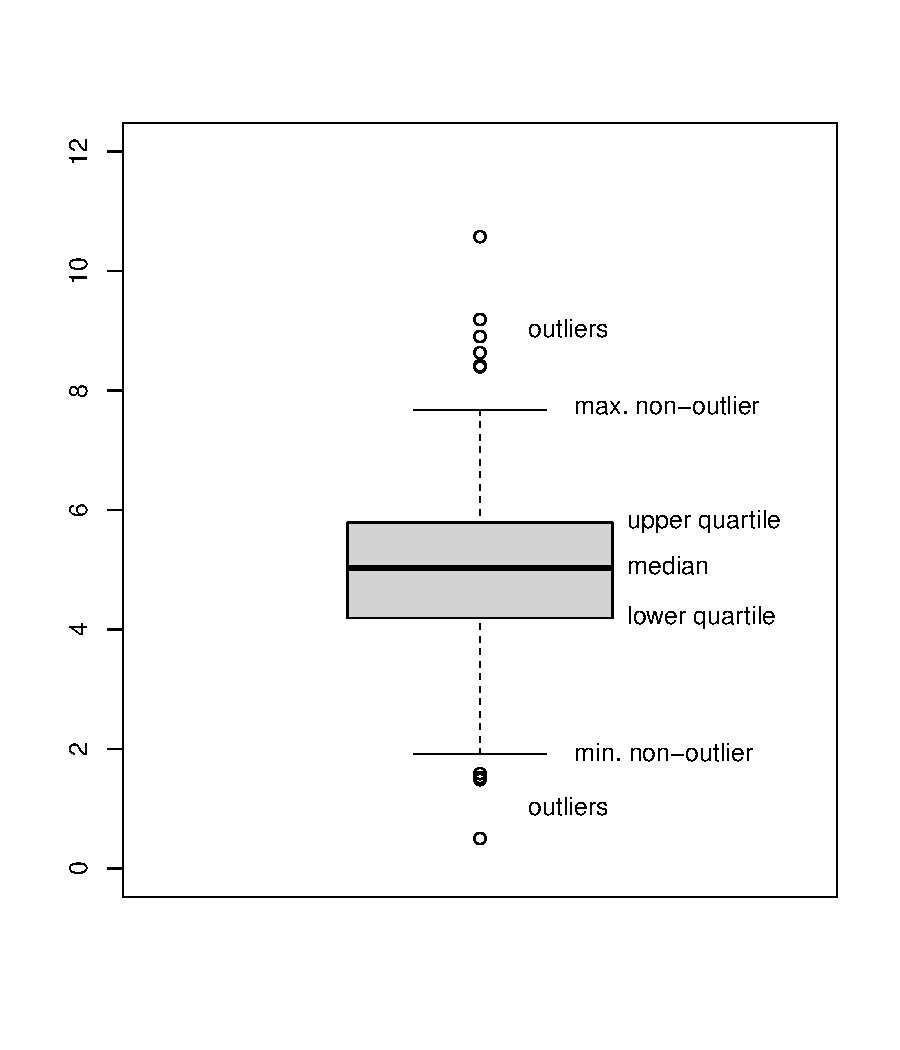
\includegraphics{math1710_files/figure-latex/boxplot1-1} \end{center}

When we have multiple datasets, drawing boxplots next to each other can help us to compare the datasets. Here are two boxplots from the July and October temperature data we used in the last lecture. What do you conclude about the data from these boxplots?

\begin{Shaded}
\begin{Highlighting}[]
\FunctionTok{boxplot}\NormalTok{(jul}\SpecialCharTok{$}\NormalTok{temp, oct}\SpecialCharTok{$}\NormalTok{temp,}
        \AttributeTok{names =} \FunctionTok{c}\NormalTok{(}\StringTok{"July"}\NormalTok{, }\StringTok{"October"}\NormalTok{),}
        \AttributeTok{ylab =} \StringTok{"Daily maximum temperature (degrees C) in Leeds"}
\NormalTok{)}
\end{Highlighting}
\end{Shaded}

\begin{center}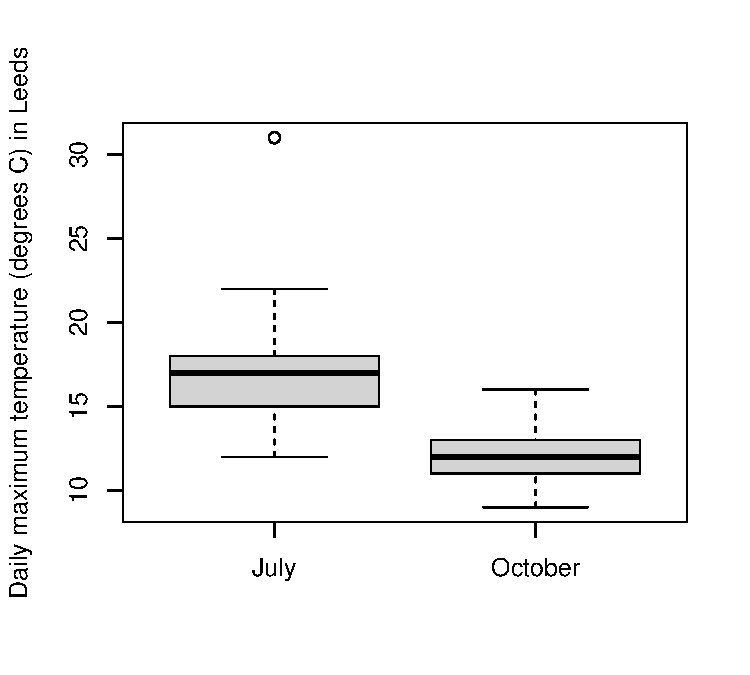
\includegraphics{math1710_files/figure-latex/boxplot-temp-1} \end{center}

(And yes, I \href{https://www.metoffice.gov.uk/binaries/content/assets/metofficegovuk/pdf/weather/learn-about/uk-past-events/interesting/2020/2020_05_july_temperature.pdf}{did check the outlier} to make sure it was a genuine datapoint.)

\hypertarget{histograms}{%
\section{Histograms}\label{histograms}}

Often when collecting data, we don't collect exact data, but rather collect data clumped into ``bins''. For example, suppose a student wished to use a questionnaire to collect data on how long it takes people to reach campus from home; they might not ask ``Exactly how long does it take?'', but rather give a choice of tick boxes: ``0--5 minutes'', ``5--10 minutes'', and so on.

Consider the following binned data, from \(n = 100\) students:

\begin{longtable}[]{@{}ccc@{}}
\toprule()
Time & Frequency & Relative frequency \\
\midrule()
\endhead
0--5 minutes & 4 & 0.04 \\
5--10 minutes & 8 & 0.08 \\
10--15 minutes & 21 & 0.21 \\
15--30 minutes & 42 & 0.42 \\
30--45 minutes & 15 & 0.15 \\
45--60 minutes & 8 & 0.08 \\
60--120 minutes & 2 & 0.02 \\
\textbf{Total} & 100 & 1 \\
\bottomrule()
\end{longtable}

Here the \textbf{frequency} \(f_j\) of bin \(j\) is simply the number of observations in that bin; so, for example, 42 students had journey lengths of between 15 and 30 minutes. The \textbf{relative frequency} of bin \(j\) is \(f_j/n\); that is, the proportion of the observations in that bin.

Which bin would you say is the most popular -- that is, the ``modal'' bin? The bin with the most observations in it is the ``15--30 minute'' bin. But this bin covers 15 minutes, while some of the other bins only cover 5 minutes. It would be a fairer comparison to look at the \textbf{frequency density}: the relative frequency divided by the size of the bin.

\begin{longtable}[]{@{}cccc@{}}
\toprule()
Time & Frequency & Relative frequency & Frequency density \\
\midrule()
\endhead
0--5 minutes & 4 & 0.04 & 0.008 \\
5--10 minutes & 8 & 0.08 & 0.016 \\
10--15 minutes & 21 & 0.21 & 0.042 \\
15--30 minutes & 42 & 0.42 & 0.028 \\
30--45 minutes & 15 & 0.15 & 0.010 \\
45--60 minutes & 8 & 0.08 & 0.005 \\
60--120 minutes & 2 & 0.02 & 0.0003 \\
\textbf{Total} & 100 & 1 & \\
\bottomrule()
\end{longtable}

In the first row, for example, the relative frequency is 0.04 and the size of the bin is 5 minutes, so the frequency density is \(0.04/5 = 0.008\). We now see that the modal bin -- the bin with the highest frequency \emph{density} -- is in fact the ``10--15 minutes'' bin. This bin has somewhat fewer datapoints that the ``15--30 minutes'' bin, but they're squashed into a much smaller bin.

Data in bins can be illustrated with a \textbf{histogram}. A histogram has the measurement on the x-axis, with one bar across the width of each bin, where bars are drawn up to the height of the corresponding frequency density. Note that this means that the area of the bar is exactly the relative frequency of the corresponding bin.

If all the bins are the same width, frequency density is directly proportional to frequency and to relative frequency, so it can be clearer use one of those as the y-axis instead in the equal-width-bins case.

Here is a histogram for our journey-time data:

\begin{Shaded}
\begin{Highlighting}[]
\NormalTok{journeys }\OtherTok{\textless{}{-}} \FunctionTok{read.csv}\NormalTok{(}\StringTok{"https://mpaldridge.github.io/math1710/data/journeys.csv"}\NormalTok{)}
\NormalTok{bins }\OtherTok{\textless{}{-}} \FunctionTok{c}\NormalTok{(}\DecValTok{0}\NormalTok{, }\DecValTok{5}\NormalTok{, }\DecValTok{10}\NormalTok{, }\DecValTok{15}\NormalTok{, }\DecValTok{30}\NormalTok{, }\DecValTok{45}\NormalTok{, }\DecValTok{60}\NormalTok{, }\DecValTok{120}\NormalTok{)}

\FunctionTok{hist}\NormalTok{(journeys}\SpecialCharTok{$}\NormalTok{midpoint, }\AttributeTok{breaks =}\NormalTok{ bins,}
     \AttributeTok{xlab =} \StringTok{"Journey length (min)"}\NormalTok{, }\AttributeTok{ylab =} \StringTok{"frequency density"}\NormalTok{, }\AttributeTok{main =} \StringTok{""}
\NormalTok{)}
\end{Highlighting}
\end{Shaded}

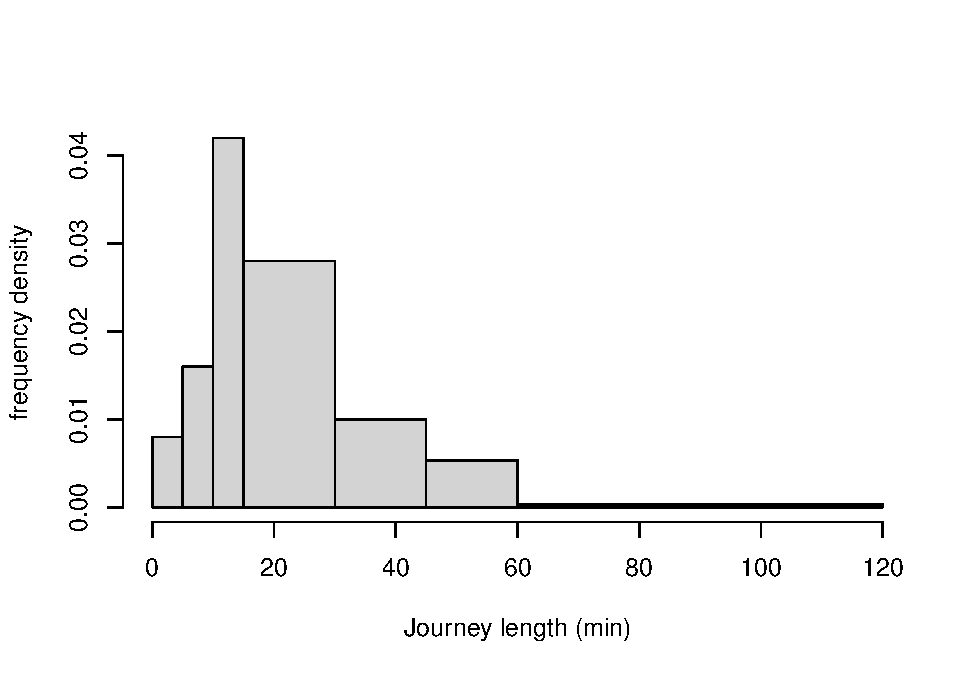
\includegraphics{math1710_files/figure-latex/journeys-1.pdf}

Often we draw histograms because the data was collected in bins in the first place. But even when we have exact data, we might \emph{choose} to divide it into bins for the purposes of drawing a histogram. In this case we have to decide where to put the ``breaks'' between the bins. Too many breaks too close together, and the small number of observations in each bin will give ``noisy'' results (see left); too few breaks too far apart, and the wide bins will mean we lose detail (see right).

\begin{Shaded}
\begin{Highlighting}[]
\FunctionTok{set.seed}\NormalTok{(}\DecValTok{2172}\NormalTok{)}
\NormalTok{hist\_data }\OtherTok{\textless{}{-}} \FunctionTok{c}\NormalTok{(}\FunctionTok{rnorm}\NormalTok{(}\DecValTok{30}\NormalTok{, }\DecValTok{8}\NormalTok{, }\DecValTok{2}\NormalTok{), }\FunctionTok{rnorm}\NormalTok{(}\DecValTok{40}\NormalTok{, }\DecValTok{12}\NormalTok{, }\DecValTok{3}\NormalTok{))  }\CommentTok{\# Some fake data}

\FunctionTok{hist}\NormalTok{(hist\_data, }\AttributeTok{breaks =} \DecValTok{40}\NormalTok{, }\AttributeTok{main =} \StringTok{"Too many bins"}\NormalTok{)}
\FunctionTok{hist}\NormalTok{(hist\_data, }\AttributeTok{breaks =} \DecValTok{2}\NormalTok{,  }\AttributeTok{main =} \StringTok{"Too few bins"}\NormalTok{)}
\end{Highlighting}
\end{Shaded}

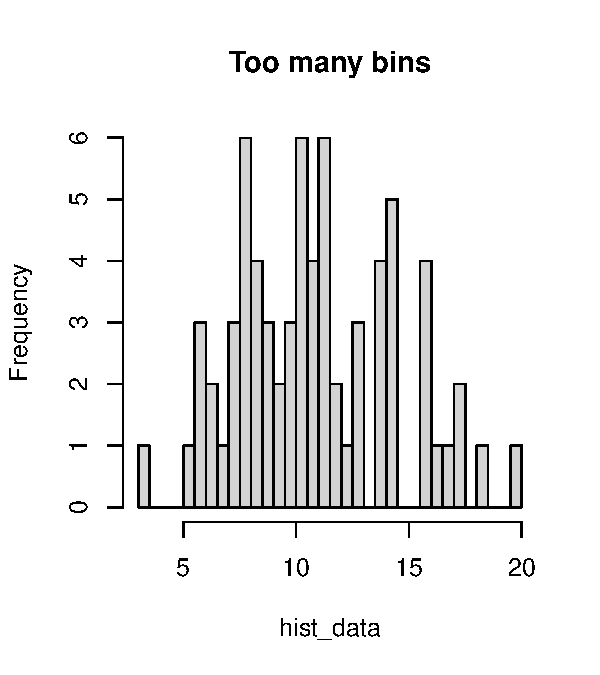
\includegraphics[width=0.48\linewidth]{math1710_files/figure-latex/hist-bins-1} 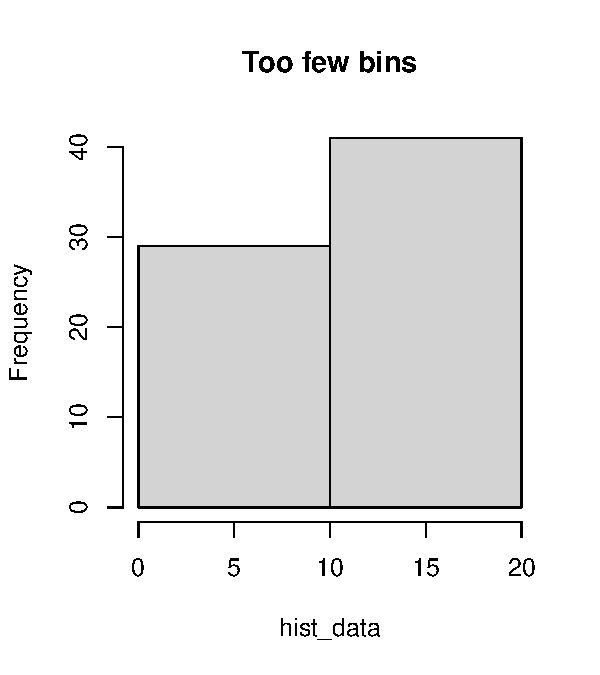
\includegraphics[width=0.48\linewidth]{math1710_files/figure-latex/hist-bins-2}

We can also calculate some summary statistics even when we have binned data. We mentioned the mode earlier, where the modal bin is the bin of highest frequency density.

What is the median journey length? Well, we don't know exactly, but \(0.04 + 0.08 + 0.21\) (the first three bins) is less than 0.5, while \(0.04 + 0.08 + 0.21 + 0.42\) (including the fourth bin) is greater than 0.5. So we know that the median student is in the fourth bin, the ``15--30 minute'' bin, and we can say that the median journey length is between 15 and 30 minutes.

Since we don't have the exact data, it's not possible to exactly calculate the mean and variance. However, we can often get a good estimate by assuming that each observation was in fact right in the centre of its bin. So, for example, we could assume that all 4 observations in the ``0--5 minutes'' bin were journeys of exactly 2.5 minutes. Of course, this isn't true (or is highly unlikely to be true), but we can often get a good approximation this way.

For our journey-time data, our approximation of the mean would be
\[ \bar x = \frac{1}{100} \big(4\times 2.5 + 8 \times 7.5 + \cdots + 2\times90) = 24.4 . \]
More generally, if \(m_j\) is the midpoint of bin \(j\) and \(f_j\) its frequency, then we can calculate the binned mean and binned variance by
\begin{align*}
  \bar x &= \frac{1}{n} \sum_j f_j m_j \\
  s^2_x  &= \frac{1}{n-1} \sum_j f_j (m_j - \bar x)^2
\end{align*}

\hypertarget{scatterplots}{%
\section{Scatterplots}\label{scatterplots}}

Often, more than one piece of data is collected from each subject, and we wish to compare that data, to see if there is a relationship between the variables.

For example, we could take \(n\) second-year maths students, and for each student \(i\), collect their mark \(x_i\) in MATH1710 and their mark \(y_i\) in MATH1712. This gives is two ``paired'' datasets, \(\mathbf x = (x_1, x_2, \dots, x_n)\) and \(\mathbf y = (y_1, y_2, \dots, y_n)\). We can calculate sample statistics of draw plots for \(\mathbf x\) and for \(\mathbf y\) individually. But we might also want to see if there is a relationship \emph{between} \(\mathbf x\) and \(\mathbf y\): Do students with high marks in MATH1710 also get high marks in MATH1712?

A good way to visualise the relationship between two variables is to use a \textbf{scatterplot}. In a scatterplot, the \(i\)th data pair \((x_i, y_i)\) is illustrated with a mark (such as a circle or cross) whose x-coordinate has the value \(x_i\) and whose y-coordinate has the value \(y_i\).

In the following scatterplot, we have \(n = 50\) datapoints for the 50 US states; for each state \(i\), \(x_i\) is the Republican share of the vote in that state in the 2016 Trump--Clinton presidential election, and \(y_i\) is the Republican share of the vote in that state in the 2020 Trump--Biden election.

\begin{Shaded}
\begin{Highlighting}[]
\NormalTok{elections }\OtherTok{\textless{}{-}} \FunctionTok{read.csv}\NormalTok{(}\StringTok{"https://mpaldridge.github.io/math1710/data/elections.csv"}\NormalTok{)}

\FunctionTok{plot}\NormalTok{(elections}\SpecialCharTok{$}\NormalTok{X2016, elections}\SpecialCharTok{$}\NormalTok{X2020,}
     \AttributeTok{col =} \StringTok{"blue"}\NormalTok{,}
     \AttributeTok{xlab =} \StringTok{"Republican share of the two{-}party vote, 2016 (\%)"}\NormalTok{,}
     \AttributeTok{ylab =} \StringTok{"Republican share of the two{-}party vote, 2020 (\%)"}\NormalTok{)}

\FunctionTok{abline}\NormalTok{(}\AttributeTok{h =} \DecValTok{50}\NormalTok{, }\AttributeTok{col =} \StringTok{"grey"}\NormalTok{)}
\FunctionTok{abline}\NormalTok{(}\AttributeTok{v =} \DecValTok{50}\NormalTok{, }\AttributeTok{col =} \StringTok{"grey"}\NormalTok{)}
\FunctionTok{abline}\NormalTok{(}\FloatTok{0.195}\NormalTok{, }\FloatTok{0.963}\NormalTok{, }\AttributeTok{col =} \StringTok{"red"}\NormalTok{)}
\end{Highlighting}
\end{Shaded}

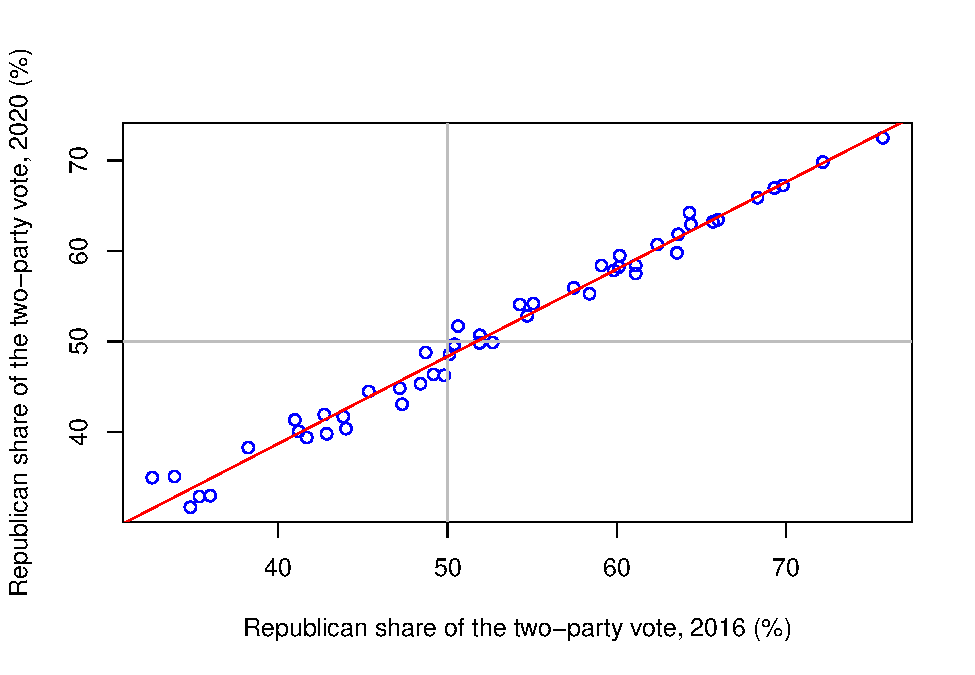
\includegraphics{math1710_files/figure-latex/elections-1.pdf}

We see that there is a strong relationship between \(\mathbf x\) and \(\mathbf y\), with high values of \(x\) corresponding to high values of \(y\) and vice versa. Further, the points on the scatterplot lie very close to a straight line.

A useful summary statistic here is the \textbf{correlation}
\[ r_{xy} = \frac{s_{xy}}{s_x s_y} , \]
where \(s_{xy}\) is the \textbf{sample covariance}
\[ s_{xy} = \frac{1}{n-1} \sum_{i=1}^n (x_i - \bar x)(y_i - \bar y) , \]
and \(s_x = \sqrt{s_x^2}\) and \(s_y = \sqrt{s_y^2}\) are the standard deviations.

The correlation \(r_{xy}\) is always between \(-1\) and \(+1\). Values of \(r_{xy}\) near \(+1\) indicate that the scatterpoints are close to a straight line with an upward slope (big \(x\) = big \(y\)); values of \(r_{xy}\) near \(-1\) indicate that the scatterpoints are close to a straight line with a downward slope (big \(x\) = small \(y\)); and values of \(r_{xy}\) near 0 indicate that there is a weak linear relationship between \(x\) and \(y\).

For the elections data, the correlation is

\begin{Shaded}
\begin{Highlighting}[]
\FunctionTok{cor}\NormalTok{(elections}\SpecialCharTok{$}\NormalTok{X2016, elections}\SpecialCharTok{$}\NormalTok{X2020)}
\end{Highlighting}
\end{Shaded}

\begin{verbatim}
## [1] 0.9919659
\end{verbatim}

which, as we expected, is extremely high.

\hypertarget{summary-02}{%
\section*{Summary}\label{summary-02}}
\addcontentsline{toc}{section}{Summary}

\begin{itemize}
\tightlist
\item
  Boxplots show the shape of numerical data, and can compare different datasets.
\item
  Histograms show the shape of binned data.
\item
  Scatterplots show the relationship between two datasets.
\end{itemize}

\hypertarget{P1}{%
\chapter*{Problem Sheet 1}\label{P1}}
\addcontentsline{toc}{chapter}{Problem Sheet 1}

\commfalse

You can \href{P1-sheet.pdf}{download this problem sheet as a PDF file}

This is Problem Sheet 1, which covers material from Lectures \protect\hyperlink{L01-stats}{1} and \protect\hyperlink{L02-dataviz}{2} of the notes. You should work through all the questions on this problem sheet in preparation for your tutorial in Week 2. Questions C1 and C2 are assessed questions, and are due in by \textbf{2pm on Monday 17 October}. I recommend spending about 4 hours on this problem sheet, plus 1 extra hour to neatly write up and submit your answers to the assessed questions.

\hypertarget{P1-short}{%
\section*{A: Short questions}\label{P1-short}}
\addcontentsline{toc}{section}{A: Short questions}

The first three questions are \textbf{short questions}, which are intended to be mostly not too difficult. Short questions usually follow directly from the material in the lectures. Here, you should clearly state your final answer, and give enough working-out (or a short written explanation) for it to be clear how you reached that answer. You can check your answers with the solutions-without-working at the bottom of this sheet; solutions-with-working will be available later. If you get stuck on any of these questions, you might want to ask for guidance in your tutorial.

\textbf{A1.} Consider again the ``number of Skittles in each packet'' data from Example 1.1.
\[ 59, \ 59, \ 59, \ 59, \ 60, \ 60, \ 60, \ 61, \ 62, \ 62, \ 62, \ 63, \ 63 .\]

\textbf{(a)} Calculate the mean number of Skittles in each packet.

\begin{myanswers}
\emph{Solution.} This was in the notes:
\[ \bar x = \frac{1}{13} (59 + 59 + \cdots + 63) =  \frac{789}{13} = 60.7 .\]

\end{myanswers}

\textbf{(b)} Calculate the sample variance using the computational formula.

\begin{myanswers}
\emph{Solution.}
\begin{align*}
s_x^2 &= \frac{1}{13 - 1} \left( (59^2 + 59^2 + \cdots + 63^2) - 13 \times 60.6923^2)\right) \\
      &= \frac{1}{12} (47915 - 47886.2) \\
      &= 2.40
\end{align*}

\textbf{Group feedback:} With the computational formula, the value \(\sum_i x_i^2 - n \bar{x}^2\) is typically a fairly small number given as the difference between two very big numbers \(\sum_i x_i^2\) and \(n \bar x^2\). This means you have to get the two big numbers very precise, to ensure the cancellation happens correctly; in particular, make sure you use plenty of decimal places of accuracy in \(\bar x\).

\end{myanswers}

\textbf{(c)} Calculate the sample variance using the definitional
formula.

\begin{myanswers}
\emph{Solution.}
\begin{align*}
s_x^2 &= \frac{1}{13 - 1} \left( (59 - 60.7)^2 + (59 - 60.7)^2 + \cdots + (63 - 60.7)^2 \right) \\
      &= \frac{1}{12} (2.86 + 2.86 + \cdots + 5.33) \\
      &= \frac{1}{12} \times 28.77 \\
      &= 2.40
\end{align*}

\end{myanswers}

\textbf{(d)} Out of (b) and (c), which calculation did you find easier, and why?

\begin{myanswers}
\emph{Solution.} The computational formula required fewer presses of the calculator buttons, because \(\sum_i x_i^2\) is fewer button-presses than \(\sum_i (x_i - \bar x)^2\), where you have to subtract the means before squaring.

On the other hand, the expression inside the brackets of the computational formula is a fairly small number given as the difference of two very large numbers, so it was necessary to use lots of decimal places of accuracy in \(\bar x\) to make sure the second large number was accurate and therefore that the subtraction cancelled correctly.

\textbf{Group feedback:} Many answer for (d) are fine provided you give a justification.

\end{myanswers}

\textbf{A2.} Consider the following data sets of the age of elected politicians on a local council. (The ``18--30'' bin, for example, means from one's
18th birthday to the moment before one's 30th birthday, so lasts 12 years.)

\begin{longtable}[]{@{}
  >{\centering\arraybackslash}p{(\columnwidth - 6\tabcolsep) * \real{0.2537}}
  >{\centering\arraybackslash}p{(\columnwidth - 6\tabcolsep) * \real{0.1642}}
  >{\centering\arraybackslash}p{(\columnwidth - 6\tabcolsep) * \real{0.2985}}
  >{\centering\arraybackslash}p{(\columnwidth - 6\tabcolsep) * \real{0.2836}}@{}}
\toprule()
\begin{minipage}[b]{\linewidth}\centering
Age (years)
\end{minipage} & \begin{minipage}[b]{\linewidth}\centering
Frequency
\end{minipage} & \begin{minipage}[b]{\linewidth}\centering
Relative frequency
\end{minipage} & \begin{minipage}[b]{\linewidth}\centering
Frequency density
\end{minipage} \\
\midrule()
\endhead
18--30 & 1 & & \\
30--40 & 3 & & \\
40--45 & 4 & & \\
45--50 & 5 & & \\
50--55 & 3 & & \\
55--60 & 1 & & \\
60--70 & 3 & & \\
\textbf{Total} & 20 & 1 & --- \\
\bottomrule()
\end{longtable}

\textbf{(a)} Complete the table by filling in the relative frequency and
frequency densities.

\begin{myanswers}

\emph{Solution.}

\begin{longtable}[]{@{}
  >{\centering\arraybackslash}p{(\columnwidth - 6\tabcolsep) * \real{0.2537}}
  >{\centering\arraybackslash}p{(\columnwidth - 6\tabcolsep) * \real{0.1642}}
  >{\centering\arraybackslash}p{(\columnwidth - 6\tabcolsep) * \real{0.2985}}
  >{\centering\arraybackslash}p{(\columnwidth - 6\tabcolsep) * \real{0.2836}}@{}}
\toprule()
\begin{minipage}[b]{\linewidth}\centering
Age (years)
\end{minipage} & \begin{minipage}[b]{\linewidth}\centering
Frequency
\end{minipage} & \begin{minipage}[b]{\linewidth}\centering
Relative frequency
\end{minipage} & \begin{minipage}[b]{\linewidth}\centering
Frequency density
\end{minipage} \\
\midrule()
\endhead
18--30 & 1 & 0.05 & 0.0041 \\
30--40 & 3 & 0.15 & 0.015 \\
40--45 & 4 & 0.2 & 0.04 \\
45--50 & 5 & 0.25 & 0.05 \\
50--55 & 3 & 0.15 & 0.03 \\
55--60 & 1 & 0.05 & 0.01 \\
60--70 & 3 & 0.15 & 0.015 \\
\textbf{Total} & 20 & 1 & --- \\
\bottomrule()
\end{longtable}

\end{myanswers}

\textbf{(b)} What is the median age bin?

\begin{myanswers}
\emph{Solution.} The 10th- and 11th-largest observations are both in the 45--50 bin, which is therefore the median bin.

\end{myanswers}

\textbf{(c)} What is the modal age bin?

\begin{myanswers}
\emph{Solution.} The bin with the largest frequency density is 45--50, which is therefore the modal bin.

\end{myanswers}

\textbf{(d)} Calculate (the standard approximation of) the mean age of the politicians.

\begin{myanswers}
\emph{Solution.} Pretending that each person is in the centre of their bin, we have
\[ \bar x = \frac{1}{20} (1\times24 + 3\times 35 + \cdots + 3 \times 65) = \frac{946.5}{20} = 47.3 . \]

\end{myanswers}

\textbf{3.} Consider the two datasets illustrated by the boxplots below. Write down some differences between the two datasets.

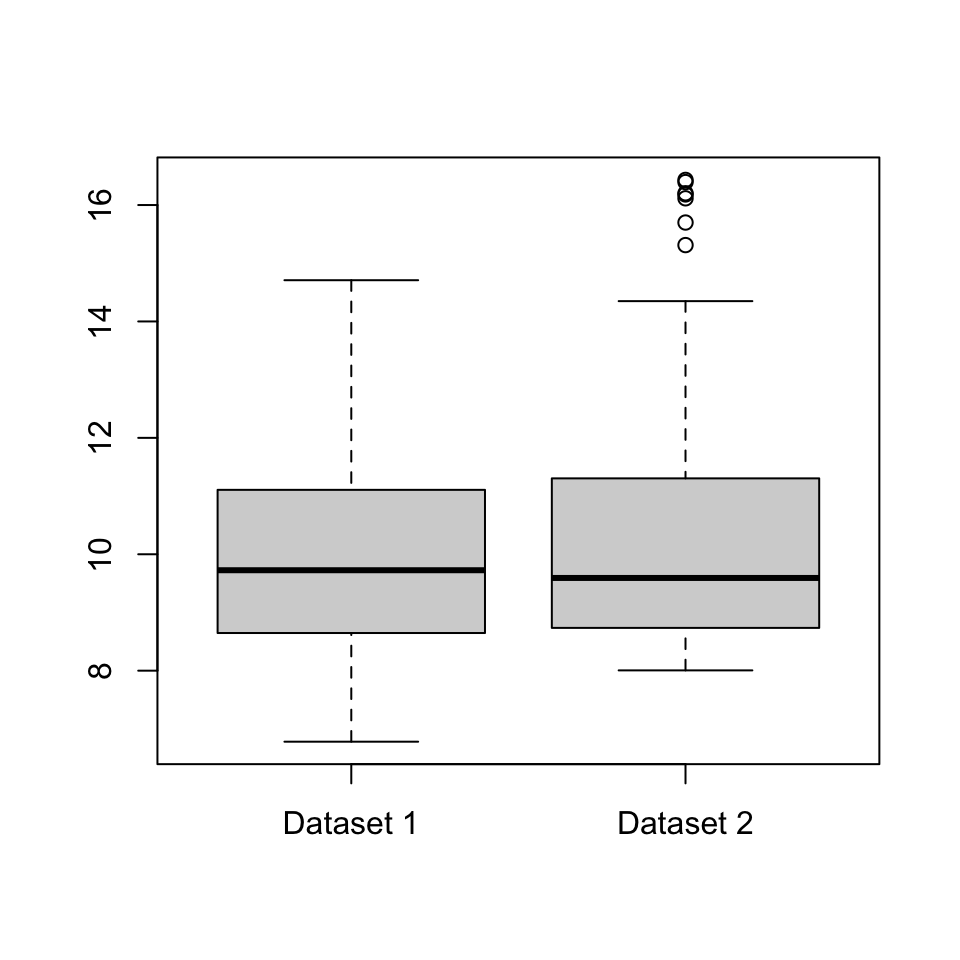
\includegraphics{math1710_files/figure-latex/two-boxplots-1.pdf}

\begin{myanswers}
\emph{Solution.} Some answers could be:

\begin{itemize}
\tightlist
\item
  The median and inter-quartile range of Dataset 2 appear to be very slightly larger than those in Dataset 1, although the differences are very small and might not be important in real life.
\item
  Dataset 2 has a few outliers; Dataset 1 has none.
\item
  While Dataset 1 is fairly ``balanced'' either side of the median, Dataset 2 shows what statisticians call a ``positive skew'': the data above the median is much more spread out than the data below the median.
\end{itemize}

\textbf{Group feedback:}
You can probably think of other answers.

\end{myanswers}

\hypertarget{P1-long}{%
\section*{B: Long questions}\label{P1-long}}
\addcontentsline{toc}{section}{B: Long questions}

The next four questions are \textbf{long questions}, which are intended to be harder. Long questions often require you to think originally for yourself, not just directly follow procedures from the notes. You may not be able to solve all of these questions, although you should make multiple attempts to do so. Here, your answers should be written in complete sentences, and you should carefully explain in words each step of your working. Your answers to these questions -- not only their mathematical content, but also how to clearly write good solutions -- are likely to be the main topic for discussion in your tutorial.

\textbf{B1.} For each of the two datasets below, calculate the following summary statistics, or explain why it is not possible to do so: mode; median; mean; number of distinct outcomes; inter-quartile range; and sample variance.

\textbf{(a)} Six packets of Skittles are opened together, and the total number of sweets of each colour is:

\begin{longtable}[]{@{}cccccc@{}}
\toprule()
\textbf{Colour} & Red & Orange & Yellow & Green & Purple \\
\midrule()
\endhead
\textbf{Number of Skittles} & 67 & 71 & 87 & 74 & 62 \\
\bottomrule()
\end{longtable}

\begin{myanswers}
\emph{Solution.}
The modal colour is Yellow. The number of distinct outcomes is 5.

It's not possible to calculate the median or the quartiles, because, unlike numerical data, the colours can't be put ``in order'' from smallest to largest.

It's not possible to calculate the mean or sample variance, as these require us to have numerical data that can be ``added up'', but this can't be done with colours.

\end{myanswers}

\textbf{(b)} Shirt sizes for a university football squad:

\begin{longtable}[]{@{}
  >{\centering\arraybackslash}p{(\columnwidth - 10\tabcolsep) * \real{0.3333}}
  >{\centering\arraybackslash}p{(\columnwidth - 10\tabcolsep) * \real{0.1667}}
  >{\centering\arraybackslash}p{(\columnwidth - 10\tabcolsep) * \real{0.1111}}
  >{\centering\arraybackslash}p{(\columnwidth - 10\tabcolsep) * \real{0.1111}}
  >{\centering\arraybackslash}p{(\columnwidth - 10\tabcolsep) * \real{0.1111}}
  >{\centering\arraybackslash}p{(\columnwidth - 10\tabcolsep) * \real{0.1667}}@{}}
\toprule()
\begin{minipage}[b]{\linewidth}\centering
\textbf{Colour}
\end{minipage} & \begin{minipage}[b]{\linewidth}\centering
Xtra Small
\end{minipage} & \begin{minipage}[b]{\linewidth}\centering
Small
\end{minipage} & \begin{minipage}[b]{\linewidth}\centering
Medium
\end{minipage} & \begin{minipage}[b]{\linewidth}\centering
Large
\end{minipage} & \begin{minipage}[b]{\linewidth}\centering
Xtra Large
\end{minipage} \\
\midrule()
\endhead
\textbf{Number of shirts} & 0 & 1 & 6 & 4 & 5 \\
\bottomrule()
\end{longtable}

\begin{myanswers}
\emph{Solution.}
The modal shirt size is medium. The number of distinct outcomes is 4 (we don't quite ``Xtra Small'', which was not observed in the data).

This time, we can order the data from smallest to largest, even though the data is not numerical. Since \((16 + 1)/2 - 8.5\), the median datapoint is the 8th or 9th datapoints, which are Large.

Since \(1 + 0.25(16 - 1) = 4.75\) the lower quartile is the 4th or 5th datapoints, which are Medium. Since \(1 + 0.75(16-1) = 12.25\), the upper quartile is the 12th or 13th datapoints, which are Xtra Large. So we can certainly say that the inner quartiles range from Medium to Xtra Large. We could probably also say that the interquartile range is 3 shirt sizes (Medium, Large, Xtra Large).

Again, because the data is not numerical, we can't add it up, so can't calculate a mean or sample variance.

\textbf{Group feedback:} Make sure your explanation is clear for why we can't calculate a median for the Skittles data but can for the shirts: they key is whether or not the data can be \emph{ordered}.

\end{myanswers}

\textbf{B2.} A summary statistic is informally said to be ``robust'' if it typically doesn't change much if a small number of outliers are introduced to a large dataset, or ``sensitive'' if it often changes a lot when a small number of outliers are introduced. Briefly discuss the robustness or sensitivity of the following summary statistics: \textbf{(a)} mode; \textbf{(b)} median; \textbf{(c)} mean; \textbf{(d)} number of distinct outcomes; \textbf{(e)} inter-quartile range; and \textbf{(f)} sample variance.

\begin{myanswers}
\emph{Solutions.}

\textbf{(a)} The mode will typically not change at all if a small number of outliers are introduced, so is robust. (The exception is for data where every observation is likely to be different, so the outliers become ``joint modes'' along with everything else; but in this case the mode is not a useful statistic in the first place.)

\textbf{(b)} The introduction of outliers will typically only change the median a little bit, by shifting it between different nearby values in the ``central mass'' of the data. In particular, the size of the outliers won't make any difference at all (only whether they are ``high outliers'' or ``low outliers''). So the median is robust.

\textbf{(c)} The mean can change a lot is outliers are introduced. (Think about the mean net worth of people in you tutorial group, and how it would change if Jeff Bezos or Elon Musk joined your tutorial group.) So the mean is sensitive.

\textbf{(d)} The number of distinct outcomes will only increase by (at most) 1 for each outlier introduced, so is robust.

\textbf{(e)} The interquartile range is robust, for the same reason as the median.

\textbf{(f)} The sample variance is sensitive, for the same reason as the mean.

(You might like to think about situations where it's better to use a robust statistic or better to use a sensitive statistic.)

\textbf{Group feedback:} Remember that ``robust'' and ``sensitive'' are general descriptions rather than precise mathematical definitions. So it doesn't matter if you disagree with my opinions provided that you give clear and detailed explanations to back up your opinion.

\end{myanswers}

\textbf{B3.} Let \(\mathbf a = (a_1, a_2, \dots a_n)\) and \(\mathbf b = (b_1, b_2, \dots, b_n)\) be two real-valued vectors of the same length. Then the \emph{Cauchy--Schwarz inequality} says that
\[ \left( \sum_{i=1}^n a_i b_i \right)^2 \leq \left( \sum_{i=1}^n a_i^2 \right) \left(\sum_{i=1}^n b_i^2 \right) . \]

\textbf{(a)} By making a clever choice of \((a_i)\) and \((b_i)\) in the Cauchy--Schwarz inequality, show that \(s_{xy}^2 \leq s_x^2 s_y^2\).

\begin{myanswers}
\emph{Solutions.}
Recalling the formulas for \(s_{xy}\), \(s_x^2\), and \(s_y^2\),
\begin{align*}
s_{xy} &= \frac{1}{n-1} \sum_{i=1}^n (x_i - \bar x)(y_i - \bar y) ,\\
s_{x}^2 &= \frac{1}{n-1} \sum_{i=1}^n (x_i - \bar x)^2 ,\\
s_{y}^2 &= \frac{1}{n-1} \sum_{i=1}^n (y_i - \bar y)^2 ,
\end{align*}
and comparing them with the Cauchy--Schwarz inequality, it looks like taking \(a_i = x_i - \bar x\) and \(b_i = y_i - \bar y\) might be useful. Making the substitution, we get
\[ \left( \sum_{i=1}^n (x_i - \bar x)(y_i - \bar y) \right)^2 \leq \left( \sum_{i=1}^n (x_i - \bar x)^2 \right) \left(\sum_{i=1}^n (y_i - \bar y)^2 \right) . \]

These are very close to the formulas for \(s_{xy}\), \(s_x^2\), and \(s_y^2\), but are just missing the ``\(1/(n-1)\)''s; what we in fact have is
\[ \left( (n-1) s_{xy} \right)^2 \leq (n-1)s_x^2 \cdot (n-1) s_y^2 .\]
Cancelling \((n-1)^2\) from each side, we have \(s_{xy}^2 \leq s_x^2 s_y^2\).

\end{myanswers}

\textbf{(b)}
Hence, show that the correlation \(r_{xy}\) satisfies \(-1 \leq r_{xy} \leq 1\).

\begin{myanswers}
\emph{Solutions.}
Recall the formula for the correlation is
\[ r_{xy} = \frac{s_{xy}}{s_xs_y} . \]
We can make part (a) look a bit like this dividing both sides by \(s_x^2 s_y^2\), to get
\[\frac{s_{xy}^2}{s_x^2 s_y^2} \leq 1.   \]
In fact that's the square of the correlation on the left-hand side, so we've shown that \(r_{xy}^2 \leq 1\).

Finally, we note that if a number squared is less than or equal to 1, then the number must be between -1 and +1 inclusive. (Numbers bigger than 1 get bigger still when squared; number smalles than -1 become bigger than +1 when squared.) Hence we have shown that \(-1 \leq r_{xy} \leq 1\), as required.

\textbf{Group feedback:} Remember that you can still attempt part (b) even if you got stuck on part (a).

\end{myanswers}

\textbf{B4.} A researcher wishes to study the effect of mental health on academic achievement. The researcher will collect data on the mental health of a cohort of students by asking them to fill in a questionnaire, and will measure academic achievement via the students' scores on their university exams. Discuss some of the ethical issues associated with the collection, storage, and analysis of this data, and with the publication of the results of the analysis. Are there ways to mitigate these issues?

(It's not necessary to write an essay for this question -- a few short bulletpoints will suffice. There may be an opportunity to discuss these issues in more detail in your tutorial.)

\begin{myanswers}
\textbf{Group feedback:} There are no ``correct'' or ``incorrect'' answers here, but here are a few things that students in my own tutorials brought up, which may act as a prompt for your own discussions.

\begin{itemize}
\tightlist
\item
  It's important the students/subjects have given their consent for their data to be used this way. It must be ``informed consent'', where they understand for what purpose the data will be used, how it will be stored, and so on. It must be possible and painless for students to decline to take part.
\item
  Consideration should be given on how to anonymise the data as much as possible -- it's not necessary for those analysing the data to know which questionnaire or which exam result belongs to which student, only that the questionnaire and results can be paired up.
\item
  Even if after data is anonymised, care should be taken about whether the students could be worked out from the data. For example, if only one student did a certain combination of modules, their identity could ``leak'' that way. Perhaps imprecise data, such as classes rather than exact marks, might help while only slightly reducing the usefulness of the data?
\item
  On one hand, it seems like this data should perhaps be deleted once analysis has been carried out, for the privacy of the students. On the other hand, principles of ``open science'' suggest that the data should be kept -- and even publically made available -- for other researchers to check the work. There are competing ethical considerations here.
\item
  If correlations are found in the data, care should be taken when publishing the analysis not to wrongly suggest a causation. (Just because X and Y are positively correlated, it doesn't mean that X \emph{causes} Y -- or that Y causes X.)
\end{itemize}

You can probably think of many other things.

\end{myanswers}

\hypertarget{P1-assessed}{%
\section*{C: Assessed questions}\label{P1-assessed}}
\addcontentsline{toc}{section}{C: Assessed questions}

The last two questions are \textbf{assessed questions}. This means you will submit your answers, and your answers will be marked by your tutor. These two questions count for 3\% of your final mark for this module. If you get stuck, your tutor may be willing to give you a small hint in your tutorial.

The deadline for submitting your solutions is \textbf{2pm on Monday 17 October} at the beginning of Week 3. Submission will be via Gradescope, which you can access via Minerva.
You should submit your answers as a single PDF file. Most students choose to hand-write their work, then scan it to PDF using their phone; if you do this, you should use a proper scanning app (like Microsoft Lens or Adobe Scan) -- please do not just submit photographs. Your work will be marked by your tutor and returned on Monday 24 October, when solutions will also be made available.

Question C1 is a ``short question'', where brief explanations or working are sufficient; Question C2 is a ``long question'', where the marks are not only for mathematical accuracy but also for the clarity and completeness of your explanations.

You should not collaborate with others on the assessed questions: your answers must represent solely your own work. The University's rules on \href{https://library.leeds.ac.uk/info/1401/academic_skills/46/academic_integrity_and_plagiarism}{academic integrity} -- and the related punishments for violating them -- apply to your work on the assessed questions.

\textbf{C1.} The monthly average exchange rate for US dollars into British pounds over a 12-month period was:
\begin{gather*}
1.306, \ 1.301, \ 1.290, \ 1.266, \ 1.268, \ 1.302,\\
1.317, \ 1.304, \ 1.284, \ 1.268, \ 1.247, \ 1.215.
\end{gather*}

\textbf{(a)} Calculate the median for this data.

\textbf{(b)} Calculate the mean for this data.

\textbf{(c)} Calculate the sample variance for this data.

\begin{myanswers}
\emph{Hints.}
Have you checked the definitions of these statistics from Subsection 1.3 of the notes?

\end{myanswers}

\textbf{(d)} Is the mode an appropriate summary statistic for this sort of data? Why/why not?

\begin{myanswers}
\emph{Hint.}
Is there a unique mode for this data? Why/why not? For what sort of data does the ``mode'' give us useful answers?

\end{myanswers}

\textbf{C2.}
~\textbf{(a)} Prove the following computational formula for the sample covariance:
\[ s_{xy} = \frac{1}{n-1} \left( \sum_{i=1}^n x_iy_i - n\bar x \bar y \right). \]

\begin{myanswers}
\emph{Hint.}
In Subsection 1.4 of the notes, we went from the definitional formula for the sample \emph{variance} to a computational formula. Can you follow a similar argument here?

\end{myanswers}

\textbf{(b)} Suppose that a dataset \(\mathbf x = (x_1, x_2, \dots, x_n)\) (with \(n \geq 2\)) has sample variance \(s_x^2 = 0\). Show that all the datapoints are in fact equal.

\begin{myanswers}
\emph{Hint.}
When is the square of something equal to 0? What can you say about the value of a square when it's nonzero? What can you say about a ``sum of squares'' -- that is, some numbers squared then added together?

\end{myanswers}

\hypertarget{P1-short-sols}{%
\section*{Solutions to short questions}\label{P1-short-sols}}
\addcontentsline{toc}{section}{Solutions to short questions}

\textbf{A1.} (a) 60.7, (b) 2.40, (c) 2.40, (d) ---. \textbf{A2.} (a) ---, (b) 45--50, (c) 45--50, (c) 47.3. \textbf{A3.} ---

\hypertarget{part-part-ii-probability}{%
\part*{Part II: Probability}\label{part-part-ii-probability}}
\addcontentsline{toc}{part}{Part II: Probability}

\hypertarget{L03-events}{%
\chapter{Sample spaces and events}\label{L03-events}}

\renewcommand{\complement}{\mathsf{c}}
\newcommand{\comp}{\complement}
\newcommand{\ff}[2]{{#1}^{\underline{#2}}}

\hypertarget{what-is-prob}{%
\section{What is probability?}\label{what-is-prob}}

We now begin the big central block of this module, on probability theory.

Probability theory is the study of randomness. Probability, as an area of mathematics, is a fascinating subject in its own right. However, probability is particularly important due to its usefulness in applications -- especially in statistics (the study of data), in finance, and in actuarial science (the study of insurance).

Probability is well suited to modelling situations that involve randomness, uncertainty, or unpredictability. If we you want to predict the time of the next solar eclipse, a deterministic (that is, non-random) model based on physical laws will tell you when the sun, the moon, and the earth will be in the correct positions; but if you want to predict the weather tomorrow, or the price of a share of Apple stock next month, or the results of an election next year, you will need a probabilistic model that takes into account the uncertainty in the outcome. A probabilistic model could tell you the most likely outcome, or a range of the most probable outcomes.

So what do we mean when we talk about the ``probability'' of an event occurring? You might say that the probability of an event is a measure of ``how likely'' it is to occur, or what the ``chance'' of it occurring is.

More concretely, here are some interpretations of probability:

\begin{itemize}
\tightlist
\item
  \textbf{Subjective} (or \textbf{Bayesian}) \textbf{probability:} The probability of an event is the way someone expresses their degree of belief that the event will occur, based on their own judgement, and given the evidence they have seen. Their belief is measured on a scale from 0 to 1, from probabilities near 0 meaning they believe the event is very unlikely to occur to probabilities near 1 meaning they believe the event is very likely to occur.

  \begin{itemize}
  \tightlist
  \item
    This interpretation is philosophically sound, but a bit vague to be the basis for a mathematics module.
  \end{itemize}
\item
  \textbf{Classical} (or \textbf{enumerative}) \textbf{probability:} Suppose there are a finite number of equally likely outcomes. Then the probability of an event is the proportion of those outcomes that correspond to the event occurring. So when we say that a randomly dealt card has a probability \(\frac{1}{13}\) of being an ace, this is because there are 52 cards of which 4 are aces, so the proportion of favourable outcomes is \(\frac{4}{52} = \frac{1}{13}\).

  \begin{itemize}
  \tightlist
  \item
    This interpretation is good for simple procedures like flipping a fair coin, rolling a dice, or dealing cards, where the ``finite number of equally likely outcomes'' assumption holds. But we want to be able to study more complicated situations, where some outcomes are more likely than others, or where infinitely many different outcomes are possible.
  \end{itemize}
\item
  \textbf{Frequentist probability:} In a repeated experiment, the probability of an event is its long-run frequency. That is, if we repeat an experiment a very large number of times, the probability of the event is (approximately) the proportion of the experiments in which the event occurs. So when we say a biased coin has probability 0.9 of landing heads, we mean that were we toss it 1000 times, we would expect to see very close to \(0.9 \times 1000 = 900\) heads.

  \begin{itemize}
  \tightlist
  \item
    There are two problems with this. First, this doesn't deal with events that can't be repeated over and over again (like ``What's the probability that England win the 2022 World Cup?''). Second, to answer the question, ``Yes, but \emph{how} close to the probability should the proportion of occurrences be?'', you end up having to answer, ``Well, it depends on the probability,'' and you've got a circular definition.
  \end{itemize}
\item
  \textbf{Mathematical probability:} We have a function that assigns to each event a number between 0 and 1, called its probability, and that function has to obey certain mathematical rules, called ``axioms''.
\end{itemize}

It will not surprise you to learn that, in this mathematics course, we will take the ``mathematical probability'' approach. However, we will also learn useful things about the other approaches: we will see that classical probability is one special case of mathematical probability; we will see a result called the ``law of large numbers'' that says that the long-run frequency does indeed get closer and closer to the mathematical probability; and a result called ``Bayes' theorem'' will advise a subjectivist on how to update her subjective beliefs when she sees new evidence.

\hypertarget{sample-events}{%
\section{Sample spaces and events}\label{sample-events}}

Taking the ``mathematical probability'' approach, we will want to give a formal mathematical definition of the \emph{probability} of an event. But even before that, we need to give a formal mathematical definition of an \emph{event} itself. Our setup will be this:

\begin{itemize}
\tightlist
\item
  There is a set called the \textbf{sample space}, normally given the letter \(\Omega\) (upper-case Omega), which is the set of all possible outcomes.
\item
  An element of the sample space \(\Omega\) is a \textbf{sample outcome}, sometimes given the letter \(\omega\) (lower-case omega), represents one of the possible outcomes.
\item
  An \textbf{event} is a set of sample outcomes; that is, a subset of the sample space \(\Omega\). Events are often given letters like \(A\), \(B\), \(C\). We write \(A \subset \Omega\) to mean that \(A\) is an event in (or, equivalently, is a subset of) the sample space \(\Omega\).
\end{itemize}

This will be easier to understand with some concrete examples. We write a set (such as a sample space or an event) by writing all the elements of that set inside curly brackets \(\{\ \}\), separated by commas.

\begin{example}
Suppose we toss a (possibly biased) coin, and record whether it lands heads or tails. Then our sample space is \(\Omega = \{\mathrm H, \mathrm T\}\), where the sample outcome H denotes heads and the sample outcome T denotes tails.

The event that the coin lands heads is \(\{\mathrm H\}\).
\end{example}

\begin{example}
Suppose we roll a dice, and record the number rolled. Then our sample space is \(\Omega = \{1,2,3,4,5,6\}\), where the sample outcome \(1\) corresponds to rolling a one, and so on.

The event ``we roll an even number'' is \(\{2,4,6\}\). The event ``we roll at least a five'' is \(\{5,6\}\).
\end{example}

\begin{example}
Suppose we wish to count how many claims are made to an insurance company in a year. We could model this by taking the sample space \(\Omega\) to be \(\mathbb Z_+ = \{0, 1, 2, \dots\}\), the set of all non-negative integers.

The event ``the company receives less than 1000 claims'' is \(\{0, 1, 2, \dots, 998, 999\}\).
\end{example}

\begin{example}
Suppose we want a computer to pick a random number between 0 and 1. We could model this by taking the sample space \(\Omega\) to be the interval \([0, 1]\) of all real numbers between 0 and 1.

The event ``the number is bigger than \(\frac12\)'' is the sub-interval \((\frac12, 1]\) of all real numbers greater than \(\frac12\) but no bigger than 1. The event ``the first digit is a 7'' is the sub-interval \([0.7, 0.8)\). The event ``the random number is exactly \(1/\sqrt{2}\)'' is \(\{1/\sqrt{2}\}\).
\end{example}

In the first two examples, the sample space \(\Omega\) was finite. In third example, the sample space was infinite but ``countably infinite'', in that it could be counted using the discrete values of the positive integers. Both of these were for \emph{counting} discrete observations. In the fourth example, the sample space was infinite but ``uncountably infinite'', in that it had a sliding scale or ``continuum'' of gradually varying measurements. This was for \emph{measuring} continuous observations. This distinction will be important later in the course.

For any sample space \(\Omega\), there are two special events that always exist. There's \(\Omega\) itself, the event containing all of the sample outcomes, which represents ``something happens''. There's also the empty set \(\varnothing\), which contains none of the sample outcomes, which represents ``nothing happens''. Common sense suggests that \(\Omega\) should have probability 1, because \emph{something} is bound to happen -- this will later be one of our probability ``axioms''. Common sense also suggests that \(\varnothing\) should have probability 0, because it can't be that \emph{nothing} happens -- this will not be one probability axioms, but we'll show that it follows logically from the axioms we do choose.

\hypertarget{set-theory}{%
\section{Set theory}\label{set-theory}}

Since we've now defined events as being sets -- specifically, subsets of the sample space \(\Omega\) -- it will be useful to mention a little set basic theory here.

First, there are ways we can build new sets (or events) out of old. It's fine to just read the words and look at the pictures for these definitions, but those who want to read the equations too will need to know this:

\begin{itemize}
\tightlist
\item
  \(\omega \in A\) means ``\(\omega\) is in \(A\)'' or ``\(\omega\) is an element of \(A\)'', while \(\omega \not\in A\) means the opposite, that \(\omega\) is \emph{not} in \(A\);
\item
  a colon \(:\) in the middle of set notation should be read as ``such that'';
\item
  so \(\{\omega \in \Omega : \text{fact about $\omega$}\}\) should be read as ``the set of sample points \(\omega\) in the sample space \(\Omega\) such that the fact is true''.
\end{itemize}

\begin{definition}

Consider a sample space \(\Omega\), and let \(A\) and \(B\) be events in that sample space.

\begin{itemize}
\tightlist
\item
  \textbf{{NOT:}} The \textbf{complement} of \(A\), written \(A^\mathsf{c}\) (and said ``\(A\) complement'' or ``not \(A\)''), is the set of sample points not in \(A\); that is
  \[ A^\mathsf{c}= \{\omega \in \Omega : \omega \not\in A \} . \]
  This represents the event that \(A\) does not occur.
\item
  \textbf{{AND}:} The \textbf{intersection} of \(A\) and \(B\), written \(A \cap B\) (and said ``\(A\) intersect \(B\)'' or ``\(A\) and \(B\)'') is the set of sample points in both \(A\) and \(B\); that is,\\
  \[ A \cap B = \{\omega \in \Omega : \omega \in A \text{ and } \omega \in B \} . \]
  This represents the event that both \(A\) and \(B\) occur.
\item
  \textbf{{OR:}} The \textbf{union} of \(A\) and \(B\), written \(A \cup B\) (and said ``\(A\) union \(B\)'' or ``\(A\) or \(B\)'') is the set of sample points in \(A\) or in \(B\); that is,
  \[ A \cup B = \{\omega \in \Omega : \omega \in A \text{ or } \omega \in B \} . \]
  This represents the event that \(A\) occurs or \(B\) occurs. (In mathematics, ``or'' includes ``both'', so a sample outcome in both \(A\) and \(B\) is in \(A\cup B\) too.)
\end{itemize}

~

\begin{center}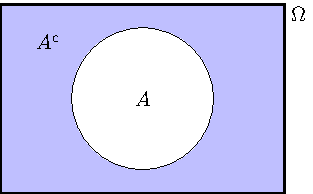
\includegraphics[width=550pt]{math1710_files/figure-latex/venn-not-1} \end{center}

\begin{center}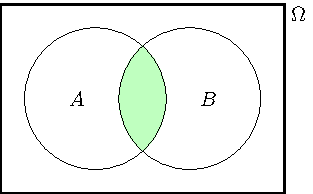
\includegraphics[width=550pt]{math1710_files/figure-latex/venn-and-1} \end{center}

\begin{center}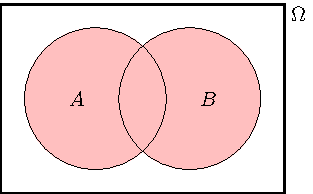
\includegraphics[width=550pt]{math1710_files/figure-latex/venn-or-1} \end{center}

\end{definition}

\begin{example}
Suppose we are rolling a dice, so our sample space is \(\Omega = \{1,2,3,4,5,6\}\). Let \(A = \{2,4,6\}\) be the event that we roll and even number, and let \(B = \{5,6\}\) be the event that we roll at least a 5. Then
\begin{align*}
A^\mathsf{c}&= \{1,3,5\} = \{\text{roll an odd number}\} ,\\
A \cap B &= \{6\} = \{\text{roll a 6}\} ,\\
A \cup B &= \{2,4,5,6\} .
\end{align*}
\end{example}

An important case is when two events \(A, B\) cannot happen at the same time; that is, \(A \cap B = \varnothing\) (``\(A\) intersect \(B\) is the empty set''). In this case, we say that \(A\) and \(B\) are \textbf{disjoint} or \textbf{mutually exclusive}. For example, when \(\Omega\) is \href{https://en.wikipedia.org/wiki/Standard_52-card_deck}{a deck of cards}, then \(A = \{\text{the card is a spade}\}\) and \(B = \{\text{the card is red}\}\) are disjoint, because a card cannot be both a spade (a black suit) and red.

There are a few rules about combining the complement, intersection and union operations.

\begin{itemize}
\tightlist
\item
  The \textbf{double complement law} tells us that not-not-\(A\) is the same as \(A\):
  \[ (A^\mathsf{c})^\mathsf{c}= A .\]
  This says that if it's not ``not-raining'', then it's raining!
\item
  The \textbf{distributive laws} tells us we can ``mutiply out of the brackets brackets'' with sets:
  \begin{align*}
  A \cap (B \cup C) &= (A \cap B) \cup (A \cap C) ,\\
  A \cup (B \cap C) &= (A \cup B) \cap (A \cup C) .
  \end{align*}
\item
  \textbf{De Morgan's laws} tell us how complements interact with intersection/unions:
  \begin{align*}
  (A \cap B)^\mathsf{c}&= A^\mathsf{c}\cup B^\mathsf{c}\\
  (A \cup B)^\mathsf{c}&= A^\mathsf{c}\cap B^\mathsf{c}
  \end{align*}
  The first of these says that if it's not a Monday in October, then either it's not Monday or it's not October (or both). The second says that if a maths lecture is not ``useful or fun'', then it's not useful and it's not fun.
\end{itemize}

If you ever do need to prove one of these statements (or a similar one), one way is to use a Venn diagram.

Let's prove the second distributive law,
\[   A \cup (B \cap C) = (A \cup B) \cap (A \cup C) , \]
with a Venn diagram as an example.

We can build the left-hand side of the law as:

\begin{center}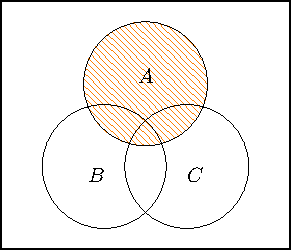
\includegraphics[width=1\linewidth]{math1710_files/figure-latex/dist1-1} \end{center}

~

\begin{center}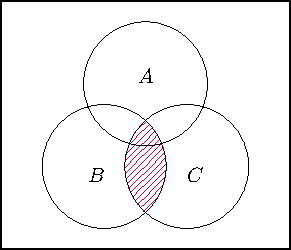
\includegraphics[width=1\linewidth]{math1710_files/figure-latex/dist2-1} \end{center}

~

\begin{center}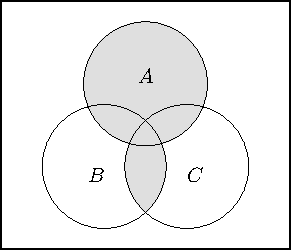
\includegraphics[width=1\linewidth]{math1710_files/figure-latex/dist3-1} \end{center}

The left-hand figure is \(\color{orange}{A}\), the middle figure is \(\color{purple}{B\cap C}\), and the right-hand figure is union of these, \(A\cup (B\cap C)\).

Then for the right-hand side of the law, we have:

\begin{center}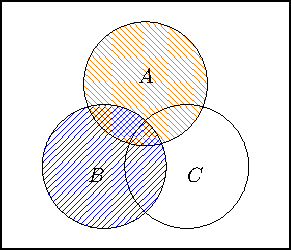
\includegraphics[width=1\linewidth]{math1710_files/figure-latex/dist4-1} \end{center}

~

\begin{center}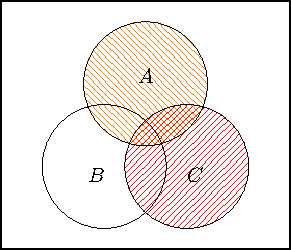
\includegraphics[width=1\linewidth]{math1710_files/figure-latex/dist5-1} \end{center}

~

\begin{center}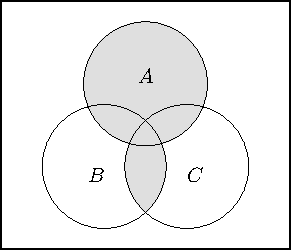
\includegraphics[width=1\linewidth]{math1710_files/figure-latex/dist6-1} \end{center}

The left-hand figure is \(\color{orange}{A} \cup \color{blue}{B}\), the middle figure is \(\color{orange}{A}\cup \color{red}{C}\), and the right-hand figure is intersection of these, \((A\cup B)\cap (A\cup C)\).

We see that the areas shaded in two right-hand figures are the same, so it is indeed the case that
\(A\cup (B\cap C) = (A\cup B)\cap (A\cup C)\).

\hypertarget{summary-L03}{%
\section*{Summary}\label{summary-L03}}
\addcontentsline{toc}{section}{Summary}

\begin{itemize}
\tightlist
\item
  A sample space \(\Omega\) is a set representing all possible sample outcomes.
\item
  An event is a subset of \(\Omega\).
\item
  For events \(A\) and \(B\), we also have the complement ``not \(A\)'' \(A^\mathsf{c}\), the intersection ``\(A\) and \(B\)'' \(A \cap B\), and the union ``\(A\) or \(B\)'' \(A \cup B\).
\end{itemize}

\hypertarget{L04-probability}{%
\chapter{Probability}\label{L04-probability}}

\hypertarget{axioms}{%
\section{Probability axioms}\label{axioms}}

Recall that, in this mathematics course, the probability of an event will be a real number that satisfies certain properties, which we call \textbf{axioms}.

\begin{definition}
\protect\hypertarget{def:axioms}{}\label{def:axioms}Let \(\Omega\) be a sample space. A \textbf{probability measure} on \(\Omega\) is a function \(\mathbb P\) that assigns to each event \(A \subset \Omega\) a real number \(\mathbb P(A)\), called the \textbf{probability} of \(A\), and that satisfies the following three axioms:

\begin{enumerate}
\def\labelenumi{\arabic{enumi}.}
\tightlist
\item
  \(\mathbb P(A) \geq 0\) for all events \(A \subset \Omega\);
\item
  \(\mathbb P(\Omega) = 1\);
\item
  if \(A_1, A_2, \dots\) is a finite or infinite sequence of disjoint events, then
  \[ \mathbb P(A_1 \cup A_2 \cup \cdots) = \mathbb P(A_1) + \mathbb P(A_2) + \cdots . \]
\end{enumerate}

The sample space \(\Omega\) together with the probability measure \(\mathbb P\) are called a \textbf{probability space}.
\end{definition}

Axiom 1 says that all probabilities are non-negative numbers. Axiom 2 says the probability that \emph{something} happens is 1. Axiom 3 says that \emph{for disjoint events} the probability that one of them happens is the sum of the individual probabilities. (Those who like their mathematical statements very precise should note that an infinite sequence in Axiom 3 must be ``countable''; that is, indexed by the natural numbers \(1, 2, 3. \dots\).)

These axioms of probability (and our later results that follow from them) were first written down by the Russian mathematician \href{https://mathshistory.st-andrews.ac.uk/Biographies/Kolmogorov/}{Andrey Nikolaevich Kolmogorov} in 1933. This marked the point from when probability theory could now be considered a proper branch of mathematics -- just as legitimate as geometry or number theory -- and not just a past-time that can be useful to help gamblers calculate their odds. I always find it surprising that the axioms of probability are less than 90 years old!

There are other properties that it seems natural that a probability measure should have aside from the axioms -- for example, that \(\mathbb P(A) \leq 1\) for all events \(A\). But we will show shortly that other properties can be proven just by starting from the three axioms.

But first, let's see some examples.

\begin{example}

Suppose we wish to model tossing an biased coin the is heads with probability \(p\), where \(0 \leq p \leq 1\).

Our probability space is \(\Omega = \{\text{H}, \text{T}\}\). The probability measure is given by
\begin{align*}
   \mathbb P(\varnothing) &= 0  &  \mathbb P(\{\text{H}\}) &= p \\
   \mathbb P(\{\text{T}\}) &= 1 - p  &  \mathbb P(\{\text{H},\text{T}\})  &= 1 .
\end{align*}

Let's check that the axioms hold:

\begin{enumerate}
\def\labelenumi{\arabic{enumi}.}
\tightlist
\item
  Since \(0 \leq p \leq 1\), all the probabilities are greater than or equal to 0.
\item
  It is indeed the case that \(\mathbb P(\Omega) = \mathbb P(\{\text{H},\text{T}\}) = 1\).
\item
  The only nontrivial disjoint union to check is \(\{\text{H}\} \cup \{\text{T}\} = \{\text{H},\text{T}\}\), where we see that
  \[ \mathbb P(\{\text{H}\}) + \mathbb P(\{\text{T}\}) = p + (1 - p) = 1 = \mathbb P(\{\text{H},\text{T}\}) , \]
  as required.
\end{enumerate}

\end{example}

\begin{example}
Suppose we wish to model rolling a dice.

Our sample space is \(\{1,2,3,4,5,6\}\). The probability measure is given by
\[ \mathbb P(A) = \frac{|A|}{6} , \]
where \(|A|\) is the number of sample outcomes in \(A\).

So, for example, the probability of rolling an even number is
\[ \mathbb P(\{2,4,6\}) = \frac36 = \frac12 . \]
\end{example}

The dice rolling is a particular case of the ``classical probability'' of equally likely outcomes. We'll look at this more in the next lecture, and prove that the classical probability measure does indeed satisfy the axioms

\hypertarget{prob-properties}{%
\section{Properties of probability}\label{prob-properties}}

The axioms of Definition \ref{def:axioms} only gave us some of the properties that we would like a probability measure to have. Our task now (in this subsection and the next) is to carefully prove how these other properties follow from just those axioms. In particular, we're not allowed to make claims that merely ``seem likely to be true'' or ``are common sense'' -- we can only use the three axioms together with strict logical deductions and nothing else.

\begin{theorem}

Let \(\Omega\) be a sample space with a probability measure \(\mathbb P\). Then we have the following:

\begin{enumerate}
\def\labelenumi{\arabic{enumi}.}
\tightlist
\item
  \(\mathbb P(\varnothing) = 0\).
\item
  \(\mathbb P(A^\mathsf{c}) = 1 - \mathbb P(A)\) for all events \(A \subset \Omega\).
\item
  For events \(A\) and \(B\) with \(B \subset A\), we have \(\mathbb P(B) \leq \mathbb P(A)\).
\item
  \(0 \leq \mathbb P(A) \leq 1\) for all events \(A \subset \Omega\).
\end{enumerate}

\end{theorem}

Importantly, the third result here tells us how to deal with complements or ``not'' events: the probability of \(A\) \emph{not} happening is 1 minus the probability it does happen. This is often very useful.

\begin{proof}
Statements 1 and 2 are exercises for you on \protect\hyperlink{P2}{Problem Sheet 2}. We'll start with the third statement.

The key with most of these ``prove from the axioms'' problems is to think of a way to write the relevant events as part of a \emph{disjoint} union, then use Axiom 3. Here, since \(B\) is a subset of \(A\), it would be useful to write \(A\) as a disjoint union of \(B\) and ``the bit of \(A\) that isn't in \(B\). That is, we have the disjoint union
\[ B \cup (A \cap B^\mathsf{c}) = A .\]

\begin{center}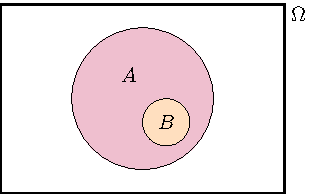
\includegraphics[width=320pt]{math1710_files/figure-latex/subs-1} \end{center}

Applying Axiom 3 to this disjoint union gives
\[ \mathbb P(B) + \mathbb P(A \cap B^\mathsf{c}) = \mathbb P(A) . \]

We're happy to see the first term on the left-hand side and the term on the right-hand side. But what about the awkward \(\mathbb P(A \cap B^\mathsf{c})\)? Well, by Axiom 1, we know that \(\mathbb P(A \cap B^\mathsf{c}) \geq 0\), and hence
\[ \mathbb P(B) + 0 \leq \mathbb P(A) , \]
and we are done with the third statement.

For the fourth statement, we have \(\mathbb P(A) \geq 0\) directly from Axiom 1, so only need to show that \(\mathbb P(A) \leq 1\). We can do this using the third statement of this theorem. For any event \(A\) we have \(A \subset \Omega\), so the third statement tells us that \(\mathbb P(A) \leq \mathbb P(\Omega)\). But Axiom 2 tells us that \(\mathbb P(\Omega) = 1\), so we are done.
\end{proof}

\hypertarget{addition}{%
\section{Addition rules for unions}\label{addition}}

If we have two or more events, we'd like to work out the probability of their union; that is, the probability that at least one of them occurs.

We already have an addition rule for \emph{disjoint} unions.

\begin{theorem}
Let \(A, B \subset \Omega\) be two disjoint events. Then
\[ \mathbb P(A \cup B) = \mathbb P(A) + \mathbb P(B) . \]
\end{theorem}

\begin{proof}
In Axiom 3, take the finite sequence \(A_1 = A\), \(A_2 = B\).
\end{proof}

But what about if \(A\) and \(B\) are not disjoint? Then we have the following.

\begin{theorem}
Let \(A, B \subset \Omega\) be two events. Then
\[ \mathbb P(A \cup B) = \mathbb P(A) + \mathbb P(B) - \mathbb P(A \cap B) . \]
\end{theorem}

You may have seen this result before. You've perhaps justified it by saying something like this: ``We can add the two probabilities together, except now we've double-counted the overlap, so we have to take the probability of that away.'' Maybe you drew a Venn diagram. That's OK as a way to remember the result -- but this is a proper university mathematics course, so we have to carefully \emph{prove} it starting from just the axioms and nothing else.

As always, the key is to find a way of writing \(A \cup B\) as a \emph{disjoint} union. (In general, \(A \cup B\) can be a non-disjoint union that has an overlap.) Well, if we want \(A \cup B = A \cup \{\text{something}\}\) to be a \emph{disjoint} union, then the ``something'' will have to be the bit of \(B\) that's not also in \(A\), which is \(B \cap A^\mathsf{c}\).

~

\begin{center}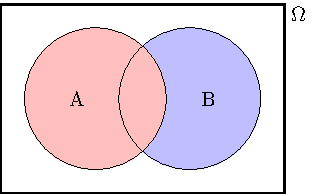
\includegraphics[width=1000pt]{math1710_files/figure-latex/add1-1} \end{center}

\begin{proof}
First note, following the discussion above, that we have
\[ A \cup B = A \cup (B \cap A^\mathsf{c}) , \]
where the union on the right is of the disjoint events \(A\) and \(B \cap A^\mathsf{c}\). Therefore we can use Axiom 3 to get
\begin{equation}
\mathbb P(A \cup B) = \mathbb P(A) + \mathbb P(B \cap A^\mathsf{c}) .    \label{eq:union1}
\end{equation}

The left-hand side looks good, and the first term on the right-hand side looks good. To deal with the second term on the right-hand side, we need to write it down as part of a disjoint union again. Can we find another one? Yes! We can use \(B \cap A^\mathsf{c}\) together with \(B \cap A\) to build the whole of \(B\). So have a disjoint union
\[ (B \cap A^\mathsf{c}) \cup (B \cap A) = B .\]

\begin{center}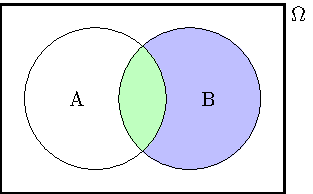
\includegraphics[width=320pt]{math1710_files/figure-latex/add2-1} \end{center}

Since this union is disjoint, we can use Axiom 3 again, to get
\[ \mathbb P(B \cap A^\mathsf{c}) + \mathbb P(B \cap A) = \mathbb P(B) . \]
Rearranging this gives
\begin{equation}
\mathbb P(B \cap A^\mathsf{c}) = \mathbb P(B) - \mathbb P(B \cap A).  \label{eq:union2}
\end{equation}

Finally, substituting \eqref{eq:union2} into \eqref{eq:union1} gives
\[ \mathbb P(A \cup B) = \mathbb P(A) + \mathbb P(B) - \mathbb P(A \cap B) , \]
as required.
\end{proof}

\begin{example}
\emph{Consider picking a card from a \href{https://en.wikipedia.org/wiki/Standard_52-card_deck}{deck} at random, with \(\mathbb P(A) = |A|/52\). What's the probability the card is a spade or an ace?}

It is possible to just to work this out directly. But let's use our addition law for unions.

We have \(\mathbb P(\text{spade}) = \frac{13}{52}\) and \(\mathbb P(\text{ace}) = \frac{4}{52}\). So we have
\[ \mathbb P(\text{spade or ace}) = \tfrac{13}{52} + \tfrac{4}{52} - \mathbb P(\text{spade and ace}) . \]
But \(\mathbb P(\text{spade and ace})\) is the probability of picking the ace of spades, which is \(\frac{1}{52}\). Therefore
\[ \mathbb P(\text{spade or ace}) = \tfrac{13}{52} + \tfrac{4}{52}  - \tfrac{1}{52} = \tfrac{16}{52} = \tfrac{4}{13} . \]
\end{example}

\hypertarget{summary-L04}{%
\section*{Summary}\label{summary-L04}}
\addcontentsline{toc}{section}{Summary}

\begin{itemize}
\tightlist
\item
  The axioms of probability are (1) \(\mathbb P(A) \geq 0\); (2) \(\mathbb P(\Omega) = 1\); and (3) that for disjoint events \(A_1, A_2, \dots\), we have \(\mathbb P(A_1 \cup A_2 \cup \cdots) = \mathbb P(A_1) + \mathbb P(A_2) + \cdots\).
\item
  Other properties can be proven from these axioms, like the complement rule \(\mathbb P(A^\mathsf{c}) = 1 - \mathbb P(A)\), and the addition rule for unions \(\mathbb P(A \cup B) = \mathbb P(A) + \mathbb P(B) - \mathbb P(A \cap B)\).
\end{itemize}

\hypertarget{part-other-stuff}{%
\part*{Other stuff}\label{part-other-stuff}}
\addcontentsline{toc}{part}{Other stuff}

\hypertarget{R}{%
\chapter*{R Worksheets}\label{R}}
\addcontentsline{toc}{chapter}{R Worksheets}

\hypertarget{r-work}{%
\section*{R worksheets}\label{r-work}}
\addcontentsline{toc}{section}{R worksheets}

Each week there will be an R worksheet to work through in your own time. I recommend spending about one hour on each worksheet, plus one extra hour for worksheets with assessed questions, for checking and submitting your solutions.

\begin{longtable}[]{@{}
  >{\centering\arraybackslash}p{(\columnwidth - 4\tabcolsep) * \real{0.0923}}
  >{\raggedright\arraybackslash}p{(\columnwidth - 4\tabcolsep) * \real{0.4769}}
  >{\centering\arraybackslash}p{(\columnwidth - 4\tabcolsep) * \real{0.4308}}@{}}
\toprule()
\begin{minipage}[b]{\linewidth}\centering
Week
\end{minipage} & \begin{minipage}[b]{\linewidth}\raggedright
Worksheet
\end{minipage} & \begin{minipage}[b]{\linewidth}\centering
Deadline for assessed work
\end{minipage} \\
\midrule()
\endhead
1 & \href{https://mpaldridge.github.io/math1710/R1.html}{\textbf{R basics}} (\href{https://mpaldridge.github.io/math1710/R1-solutions.html}{Solutions}) & --- \\
2 & \href{https://mpaldridge.github.io/math1710/R2.html}{\textbf{Vectors}} & --- \\
3 & Data in R & Monday 24 October (Week 4) \\
4 & Plots I: Making plots & --- \\
5 & Plots II: Making plots better & Monday 7 November (Week 6) \\
6 & RMarkdown (optional) & --- \\
7 & Discrete distributions & Monday 21 November (Week 8) \\
8 & Discrete random variables & --- \\
9 & Normal distribution & Monday 5 December (Week 10) \\
10 & Law of large numbers & --- \\
11 & Recap & Thursday 15 December (Week 11) \\
\bottomrule()
\end{longtable}

\hypertarget{about-r}{%
\section*{About R and RStudio}\label{about-r}}
\addcontentsline{toc}{section}{About R and RStudio}

\begin{itemize}
\tightlist
\item
  \textbf{R} is a \emph{programming language} that is particularly useful for working with probability and statistics. R is very widely used in universities and increasingly widely used in industry. Learning to use R is a mandatory part of this module, and exercises requiring use of R make up at least 15\% of your module mark. Many other statistics-related modules at the University also use R.
\item
  \textbf{RStudio} is a \emph{program} that gives a convenient way to work with the language R. RStudio is the most common way to use the language R, and learning to use RStudio is strongly recommended.
\end{itemize}

R and RStudio are free/open-source software.

\hypertarget{r-access}{%
\section*{How to access R and RStudio}\label{r-access}}
\addcontentsline{toc}{section}{How to access R and RStudio}

There are a few ways you can access R and RStudio.

First, you can \textbf{install R and RStudio on your own computer}. Students who have their own computer (with administration and installation rights) usually find this the most convenient way use R.

When you install R and RStudio, it's important that you install R (the programming language) first, and only install RStudio (the program to use R) after R has already been installed. This ensures that RStudio can ``find'' R on your computer.

\begin{enumerate}
\def\labelenumi{\arabic{enumi}.}
\item
  \emph{First}, install R. Go to the \href{https://cran.r-project.org/}{Comprehensive R Archive Network (CRAN)} and follow the instructions:

  \begin{itemize}
  \tightlist
  \item
    Windows: Click \href{https://cran.r-project.org/bin/windows/}{``Download R for Windows''}, then \href{https://cran.r-project.org/bin/windows/base/}{``Install R for the first time''}. The main link at the top should be to download the most recent version of R.
  \item
    Mac: Click \href{https://cran.r-project.org/bin/macosx/}{Download R for macOS}, and then download the relevant PKG file. (For typically older Intel-based Macbooks, you must use the ``Intel 64-bit build''; for post-November 2020 M1 or M2-based ``Apple silicon'' Macbooks, the ``Apple silicon arm64 build'' may be slightly faster.)
  \end{itemize}
\item
  \emph{After} R is installed, \emph{then} install RStudio. Go to \href{https://www.rstudio.com/products/rstudio/download/\#download}{the Download page at RStudio.com} and follow the instructions. You want ``RStudio Desktop'', and you want the free version.
\end{enumerate}

If you have difficulty installing R, come along to the R troubleshooting drop-in session in Week 2 and bring your computer with you (if it's sufficiently portable), and we'll do our best to help.

Second, you can \textbf{use R and RStudio on University computers}. All University computers have access to R and RStudio, via the AppsAnywhere service. Again, you should first install R (which, at the time of writing, is confusingly included under the name ``CRAN R'') via AppsAnywhere, and then install RStudio via AppsAnywhere.

The R drop-in sessions take place in computer rooms, so if you have problems accessing R and RStudio on University computers, you can get help at the drop-in sessions too.

Third, you can \textbf{use the \href{https://rstudio.cloud/}{RStudio Cloud}}. The RStudio Cloud is a cloud-hosted ``Google Docs for R'' that you can use through your web browser, without having to install anything. You can get 25 hours per month for free, which should be plenty for this module, or pay for more.

If you have access to a computer on which you can't install software, such as some Chromebooks or tablet computers, or if you're borrowing a friend's laptop, the RStudio Cloud can be a convenient solution.

\hypertarget{troubleshooting}{%
\section*{R troubleshooting drop-in sessions}\label{troubleshooting}}
\addcontentsline{toc}{section}{R troubleshooting drop-in sessions}

You will learn to use R by working through the R Worksheets. Learning to use a programming language is different from learning mathematics: you should expect to regularly get frustrated and annoyed when the computer seems to refuse to do what you want it to (but also occasionally experience the joy of getting it right!). This is a normal part of learning.

However, many students find getting with started with R in the first few weeks particularly difficult. Also, sometimes students have problems installing R and RStudio on their own computers. To help with this, we have organised optional R troubleshooting drop-in sessions in Weeks 2 and 3. Check your timetable for details -- they are probably listed as ``computer practicals''.

\end{document}
